\chapter{Continuous Integration with Jenkins}
\ChapterLabel{Jenkins}
\index{Jenkins}
\index{continuous integration}
\index{merge gate}

\section{Overview and Status}
This chapter answers the course manual's Chapter~4 \cite{DosManual}: a Gitea pull request
on the startup's product repository \texttt{twintrack} starts a Jenkins pipeline, Jenkins
reports a named status on the proposed commit, and Gitea refuses the merge while that
required check fails. Jenkins runs as a controlled service on the same AWS EC2 instance as
Gitea. The eight numbered subsections match the eight rubric rows in order. Evidence is
dated November 2, 2026 (US Eastern) unless stated otherwise; the Jenkins log times are in UTC
and fall on November 3.

\begin{tabularx}{\linewidth}{L{5.6cm}L{1.4cm}L{1.6cm}Y}
\caption{Rubric rows, owners, and status\label{Table:JenkinsStatus}}\\
\toprule \textbf{Subsection} & \textbf{Points} & \textbf{Owner} & \textbf{Status}\\ \midrule
\endfirsthead
\toprule \textbf{Subsection} & \textbf{Points} & \textbf{Owner} & \textbf{Status}\\ \midrule
\endhead \bottomrule \endlastfoot
Jenkins deployment and persistence & 10 & BD & \StatusPass\\
HTTPS, access, and firewall & 15 & BD & \StatusPass\\
Gitea trigger and traceability & 15 & BD & \StatusPass\\
Versioned pipeline and tests & 15 & SD (draft BD, checked SD) & \StatusPass\\
Required merge gate & 15 & SD (draft BD, checked SD) & \StatusPass\\
Failure, repair, and review & 10 & SD (draft BD, checked SD) & \StatusPass\\
Credentials and build boundary & 10 & BD & \StatusPass\\
Manual quality and controls & 10 & SD (draft BD, checked SD) & \StatusPass\\
\end{tabularx}

\paragraph{Key facts.} Jenkins: \href{https://ci.ssw590-g1.tech/login}{\texttt{https://ci.ssw590-g1.tech/login}}.
Product repository: \href{\GiteaURL/group1-startup/twintrack}{\texttt{group1-startup/twintrack}};
pull request \href{\GiteaURL/group1-startup/twintrack/pulls/10}{\#10} closes issue
\href{\GiteaURL/group1-startup/twintrack/issues/9}{\#9}. Required status check on \texttt{main}:
\textbf{\texttt{twintrack/pipeline/pr-main}}. Deployment files:
\href{\GiteaURL/group1-startup/infra/src/branch/main/jenkins}{\texttt{group1-startup/infra}, folder \texttt{jenkins}}.

\section{Required Subsections}
% ======================================================================
% Region: jenkDeployment (single owner; edit only your own region)
\subsection{Jenkins deployment and persistence (10 points)}
\label{Section:jenkDeployment}
\textbf{Owner:} BD. \textbf{Status:} deployed, restarted, and verified on November 2, 2026 \StatusPass.

\paragraph{What runs.} Jenkins is an official LTS image, \texttt{jenkins/jenkins:2.580.2-lts-jdk21} from
Docker Hub \cite{JenkinsDocker}. The tag is pinned to an exact version (it was the newest 2.580 LTS tag,
published October 28, 2026, about 244~MB for amd64) and was not \texttt{lts} or \texttt{latest}. A thin
local \texttt{Dockerfile} adds \texttt{python3}, because the course's example \texttt{Jenkinsfile} runs
Python tests on the controller executor, and installs the plugins at build time so the plugin versions are
part of the image (\ListRef{72}). The file set is in the \texttt{infra} repository,
\href{\GiteaURL/group1-startup/infra/src/branch/main/jenkins}{folder \texttt{jenkins}}; the sources are also printed
below. No password, token, or key is in any of them.

\begin{longlisting}
\inputminted[fontsize=\scriptsize]{docker}{config/jenkins/Dockerfile}
\caption{\texttt{Dockerfile} of the Jenkins image: official LTS image, \texttt{python3}, and four plugins (their dependencies are resolved at build time).}
\label{Listing:JenkinsDockerfile}
\end{longlisting}

\begin{longlisting}
\inputminted[fontsize=\scriptsize]{yaml}{config/jenkins/docker-compose.yml}
\caption{Compose file: no \texttt{ports:} on purpose, a 640~MiB memory limit, a 384~MB Java heap, a named volume, and the Docker network that Gitea and Caddy already share.}
\label{Listing:JenkinsCompose}
\end{longlisting}

\begin{tabularx}{\linewidth}{L{3.6cm}Y}
\caption{Jenkins deployment record\label{Table:JenkinsRecord}}\\
\toprule \textbf{Property} & \textbf{Value}\\ \midrule
\endfirsthead
\toprule \textbf{Property} & \textbf{Value}\\ \midrule
\endhead \bottomrule \endlastfoot
Image and versions & \texttt{group1/jenkins-python:2.580.2}, built on the host from \texttt{jenkins/jenkins:2.580.2-lts-jdk21}; Jenkins 2.580.2, OpenJDK 21.0.13, Python 3.13.5; 547~MB (\ListRef{72})\\
Key plugins (versions) & \texttt{gitea} 286.v0740a\_413c1eb\_, \texttt{git} 5.11.0, \texttt{workflow-aggregator} (Pipeline) 608.v67378e9d3db\_1, \texttt{matrix-auth} 3.3; the complete list of 60 installed plugins with versions is in \ListRef{72}\\
Host capacity & AWS EC2 \texttt{t3.micro}: 913~MB RAM, 2~GB swap, 20~GB disk (about 9.3~GB free). The same host runs Gitea, Caddy, and the Assignment~5 runner\\
Limits & Container limit 640~MiB (swap up to 1~GB); Java heap \texttt{-Xms128m -Xmx384m}; if Jenkins outgrows its limit only the Jenkins container is killed, not Gitea\\
Persistent volume & Named volume \texttt{jenkins\_jenkins\_home} mounted at \texttt{/var/jenkins\_home}: settings, accounts, credentials, jobs, and build history\\
Restart policy & \texttt{restart: unless-stopped}\\
Network & Joins the existing \texttt{gitea\_web} network; \textbf{no published ports}, so neither 8080 nor the agent port 50000 exists on the host\\
Deployment command & \texttt{docker compose up -d --build} in \texttt{\textasciitilde/jenkins} on the server\\
\end{tabularx}

\paragraph{Capacity decision and first start.} The server is small, so the decision to place Jenkins beside
Gitea (instead of resizing or adding an instance) was made on October 29, 2026 with a rule: resize only if
Jenkins is killed for memory, swap stays above about 1~GB, or Gitea slows. The image was built with a watchdog
that would abort at 1~GB of swap or an unhealthy Gitea; it did not trigger (lowest free memory 131~MB, swap
peak 147~MB). Jenkins started and logged ``fully up and running'' about 25~seconds after the start, peaking at
408~MiB of its 640~MiB limit, and once settled the machine had about 98~MB of RAM free with swap absorbing the
rest (\ListRef{73}). It fits, but with little headroom; later checks during builds showed 91--213~MB free and
swap use between 187 and 531~MB, with Gitea healthy throughout.

\paragraph{Restart test.} On November 2, 2026 the container was restarted with \texttt{docker compose restart
jenkins}. The two named accounts, the global configuration (which holds the matrix security settings and the Jenkins
URL), the credentials store, the multibranch job, and the build history (builds 1 to 5) have the \emph{same
checksums} before and after, and the service answered again about 12.6~seconds later (log line ``fully up and
running'' at 00:44:03 UTC after the restart at 00:43:50 UTC); anonymous \texttt{/login} returned HTTP~200 and the API
stayed refused (\ListRef{102}). A first reading of ``9~seconds'' was wrong (its log filter matched the previous start)
and is corrected in that file. \textbf{This is a persistence test, not a backup test:} the data stays on the same server
disk, and the optional backup and restore of Chapter~\ref{Chapter:Gitea} was not attempted.

\begin{longlisting}
\inputminted[fontsize=\scriptsize]{text}{evidence/72-jenkins-image-build-and-plugin-versions-2026-10-29.txt}
\caption{Image build on the server (exit code 0, 547~MB), memory watchdog, and the 60 plugins with exact versions, October 29, 2026 (real output).}
\label{Listing:E72}
\end{longlisting}

\begin{longlisting}
\inputminted[fontsize=\scriptsize]{text}{evidence/73-jenkins-first-start-memory-and-exposure-2026-10-29.txt}
\caption{First start: time to ready, memory, no published ports, private reachability from Caddy, and raw port 8080 closed from outside, October 29, 2026 (real output).}
\label{Listing:E73}
\end{longlisting}

\begin{longlisting}
\inputminted[fontsize=\scriptsize]{text}{evidence/102-jenkins-container-restart-test-before-after-2026-11-02.txt}
\caption{Restart test: state before and after (identical checksums), readiness time, and the correction of a wrong first reading, November 2, 2026 (real output).}
\label{Listing:E102}
\end{longlisting}

\begin{figure}[htbp]
\centering
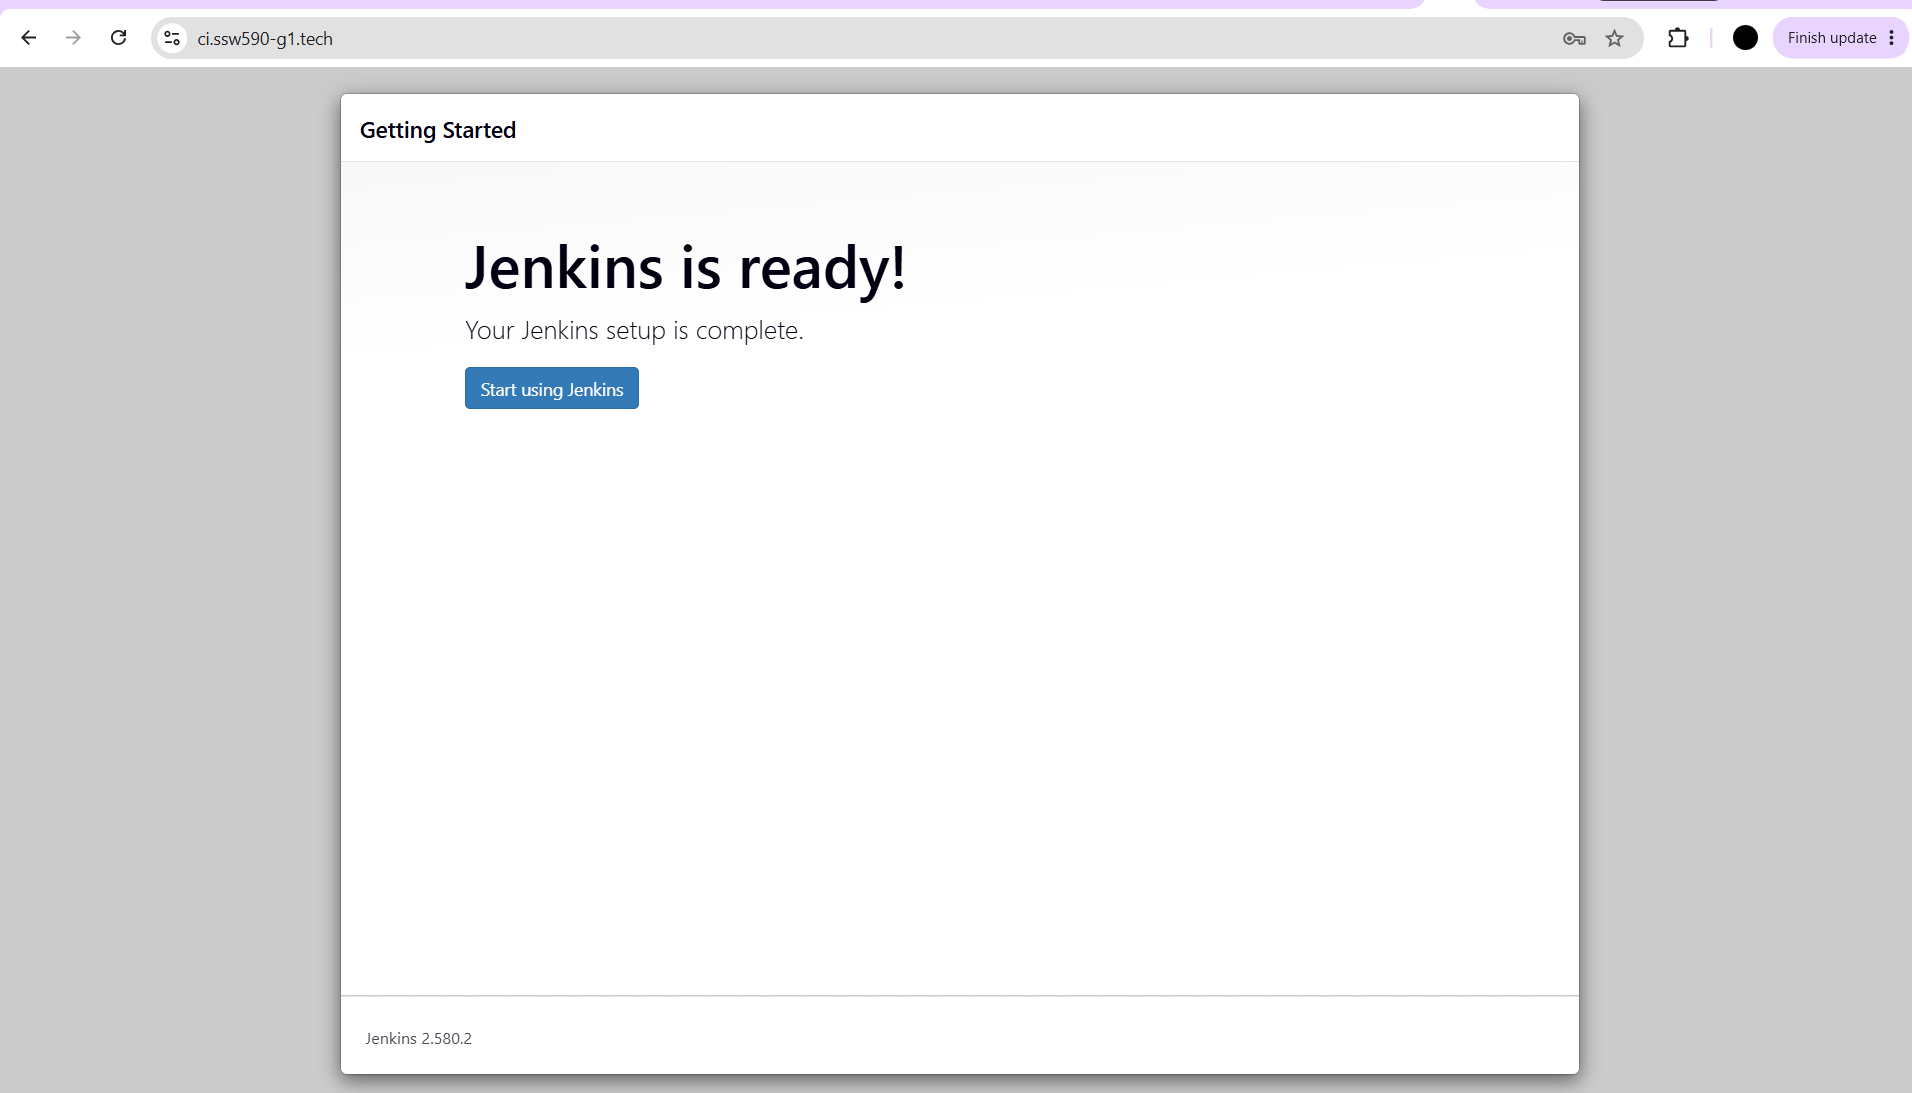
\includegraphics[width=0.8\linewidth]{evidence/78-jenkins-setup-wizard-complete-ready-2.580.2-2026-11-02.png}
\caption{First-time setup finished, November 2, 2026: ``Jenkins is ready! Your Jenkins setup is complete'', Jenkins 2.580.2. The one-time unlock password was read on the server and is not shown.}
\label{Fig:E78}
\end{figure}

% ======================================================================
% Region: jenkAccess (single owner; edit only your own region)
\subsection{HTTPS, access, and firewall (15 points)}
\label{Section:jenkAccess}
\textbf{Owner:} BD. \textbf{Status:} live and tested from outside, IPv4 only \StatusPass.

\paragraph{Login page and the instructor's access path.}
The complete, working URL of the Jenkins login page is
\href{https://ci.ssw590-g1.tech/login}{\texttt{https://ci.ssw590-g1.tech/login}}. \textbf{No account is needed to open
it.} Caddy lets \emph{anyone} open exactly the login page and the few static files it needs; every other path
(\texttt{/}, the dashboard, the API) answers a plain \emph{Forbidden} unless the request comes from the team's approved
address. So the instructor opens the URL in any browser and sees the sign-in page (\FigRef{105}); to inspect the rest
of Jenkins a team member signs in from the approved address. \emph{This check shows that the web service is available;
it does not show that a pipeline works}, which is shown in the following subsections. The phone test in \FigRef{76}
(left and right images) was made on mobile data, outside the team address: the Jenkins page opened without an account (it was
still the first-time unlock screen then) and \texttt{/} answered \emph{Forbidden}.

\begin{figure}[htbp]
\centering
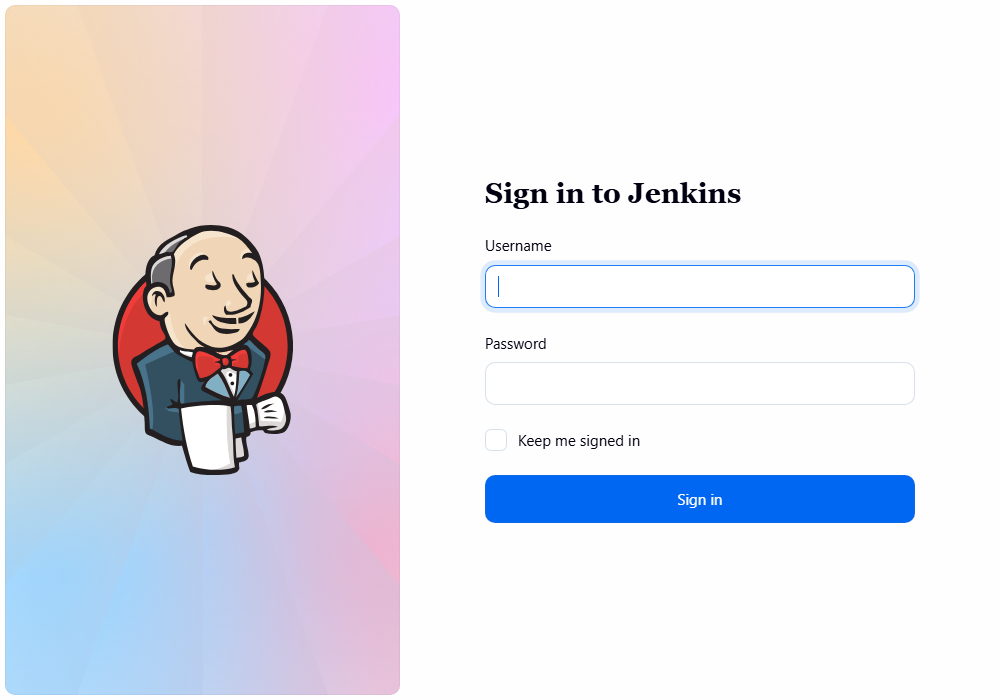
\includegraphics[width=0.85\linewidth]{evidence/105-jenkins-login-page-sign-in-public-url-headless-chrome-2026-11-02.png}
\caption{The public login page \texttt{https://ci.ssw590-g1.tech/login} on November 2, 2026 (captured with headless Chrome from the administrator's computer): ``Sign in to Jenkins'', username, password, and Sign in.}
\label{Fig:E105}
\end{figure}

\begin{figure}[htbp]
\centering
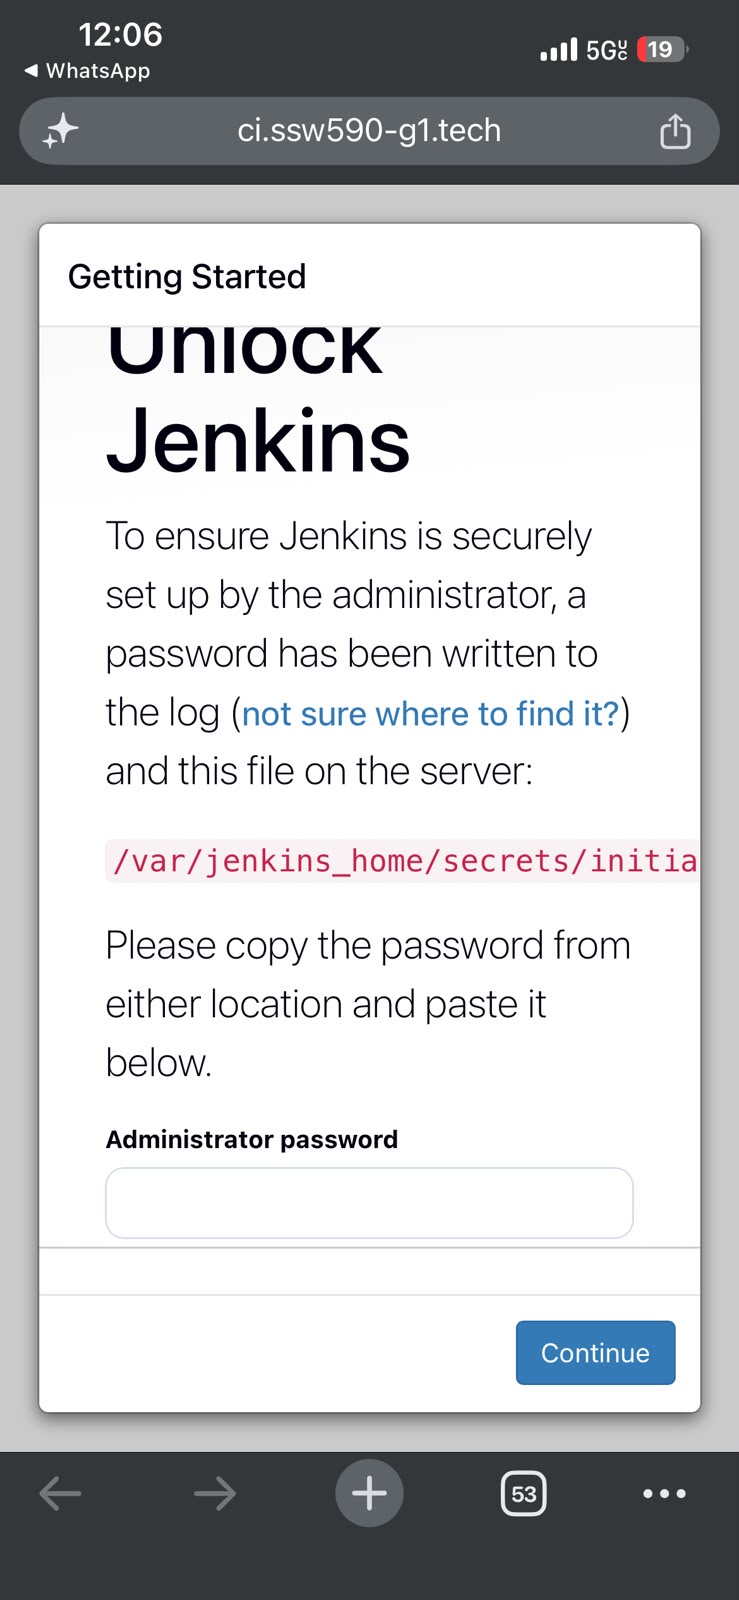
\includegraphics[width=0.38\linewidth]{evidence/76-phone-mobile-data-ci-login-page-opens-unlock-jenkins-2026-11-02.jpg}\hfill
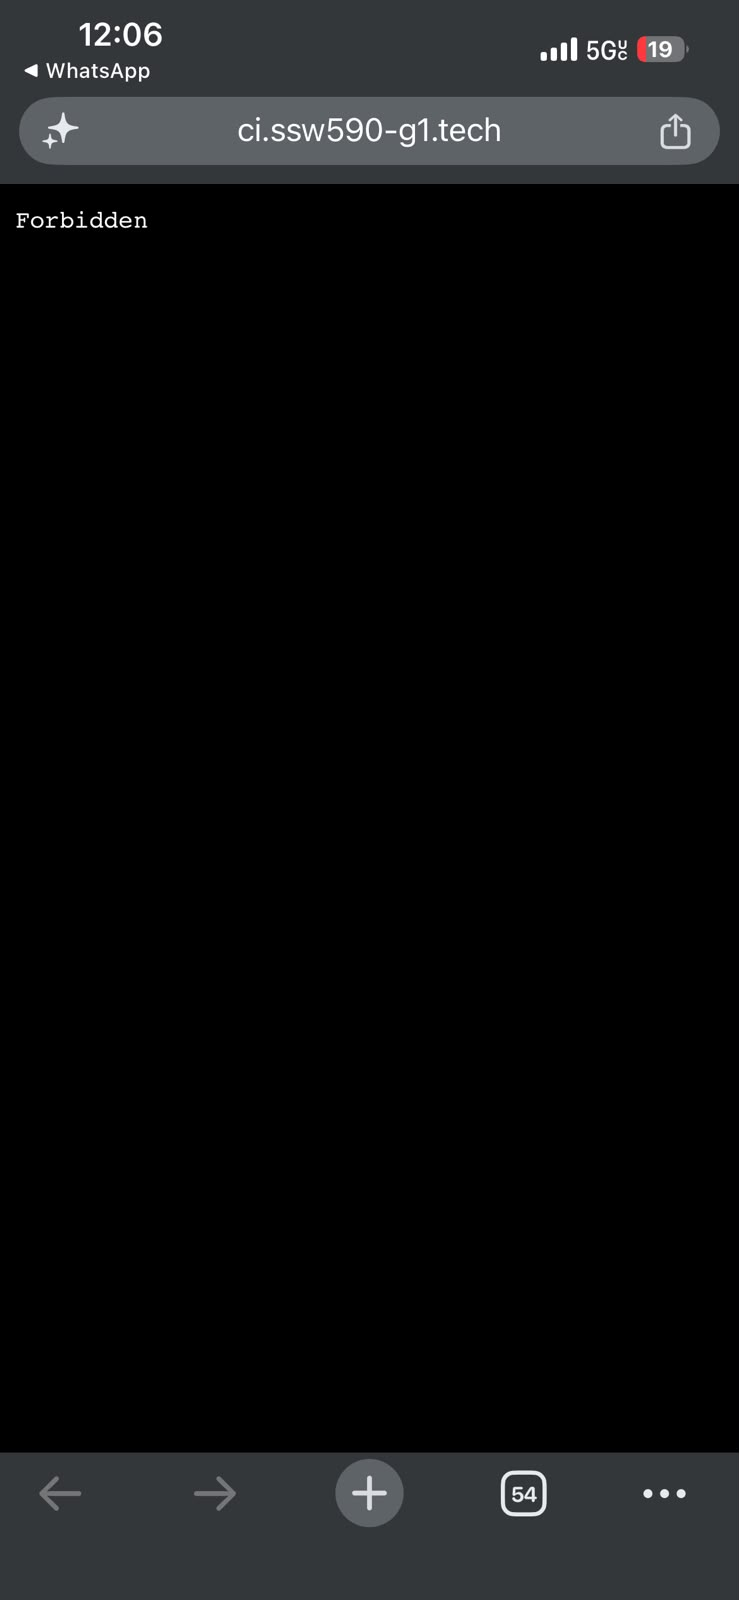
\includegraphics[width=0.38\linewidth]{evidence/77-phone-mobile-data-ci-root-forbidden-2026-11-02.jpg}
\caption{External test from a phone on mobile data, November 2, 2026, 12:06 PM. Left: the Jenkins page opens without an account (the first-time ``Unlock Jenkins'' screen, because setup was not finished yet). Right: \texttt{https://ci.ssw590-g1.tech/} answers \emph{Forbidden}.}
\label{Fig:E76}
\end{figure}

\paragraph{DNS and certificate.} An A record \texttt{ci.ssw590-g1.tech} points to the same Elastic IP as the Gitea host
(TTL 300, created November 1, 2026; \FigRef{74}); no AAAA record exists. Caddy obtained a Let's Encrypt certificate for the new name
automatically on its first request (TLS-ALPN-01 on port 443). It is valid from \textbf{November 2, 2026 04:04 UTC to
January 31, 2027 04:04 UTC}, issuer \texttt{CN=YE2, O=Let's Encrypt}, with a valid chain (\ListRef{75}). HTTP is
redirected to HTTPS with a 308. \textbf{Renewal} uses the same automatic mechanism and the same Caddy instance and storage
volume as the Gitea certificate (\ChapterRef{Gitea}); the staging dry-run described there covers it. The first real renewal of this
certificate (due before January 31, 2027) has not happened yet and is not claimed.

\begin{figure}[htbp]
\centering
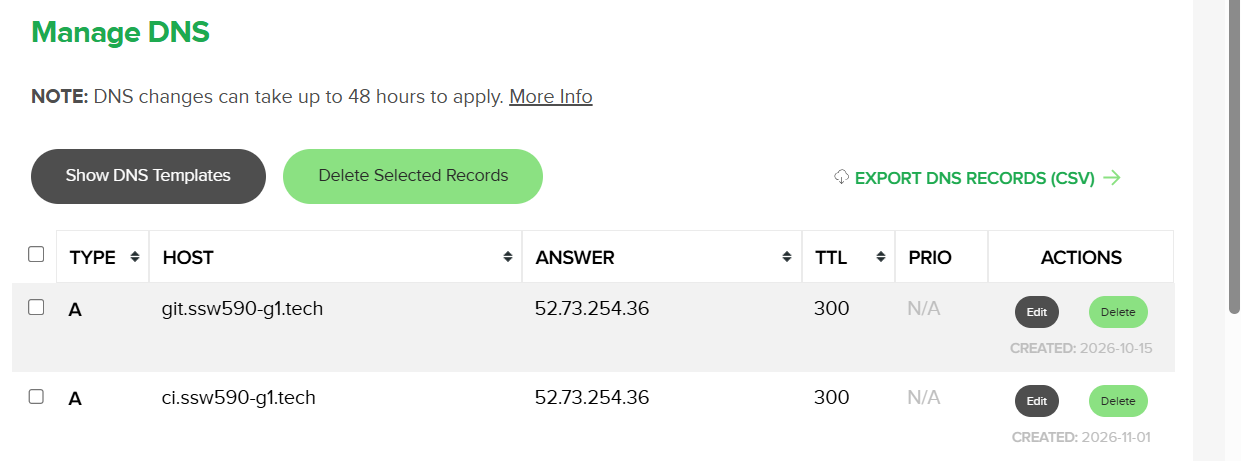
\includegraphics[width=\linewidth]{evidence/74-namecom-dns-a-record-ci-ssw590-g1-tech-2026-11-01.png}
\caption{Name.com Manage DNS, November 1, 2026: new A record \texttt{ci.ssw590-g1.tech} to the same address as \texttt{git.ssw590-g1.tech}, TTL 300.}
\label{Fig:E74}
\end{figure}

\paragraph{Caddy, the Jenkins URL, and proxy settings.} Caddy terminates TLS and proxies to the container by service
name (\ListRef{75} shows the change and the new site block); it was applied with a backup of the old Caddyfile and compose
file and an automatic rollback, and only the Caddy container was recreated (Gitea stayed healthy). The team's
address list lives only in the server's untracked \texttt{.env} (mode 600), never in the repository. The Jenkins URL is
\texttt{https://ci.ssw590-g1.tech/} (read from the saved configuration in \ListRef{102}). Caddy's reverse proxy adds
the forwarding headers itself; a screenshot of Jenkins' ``reverse proxy setup'' check was not captured, so that
check is not claimed.

\begin{longlisting}
\inputminted[fontsize=\scriptsize]{text}{evidence/75-caddy-ci-block-applied-certificate-and-first-http-checks-2026-11-02.txt}
\caption{Caddy change with backups and rollback prepared, certificate for the new name, and the first HTTP/HTTPS checks, November 2, 2026 (real output; the allowed address is never printed).}
\label{Listing:E75}
\end{longlisting}

\paragraph{Named accounts and roles.} Registration is closed (\emph{Allow users to sign up} is off). There are two
named accounts in Jenkins' own user database, \texttt{brahmi} and \texttt{sakshi} (\FigRef{79}). Authorization uses
\emph{Matrix-based security}: Brahmi has \emph{Overall Administer}; Sakshi has Overall Read, Job Build and Read, and
View Read; \emph{Anonymous} and \emph{Authenticated Users} have no permissions (\FigRef{80}). Anonymous requests to
the API are refused (HTTP 403).

\begin{figure}[htbp]
\centering
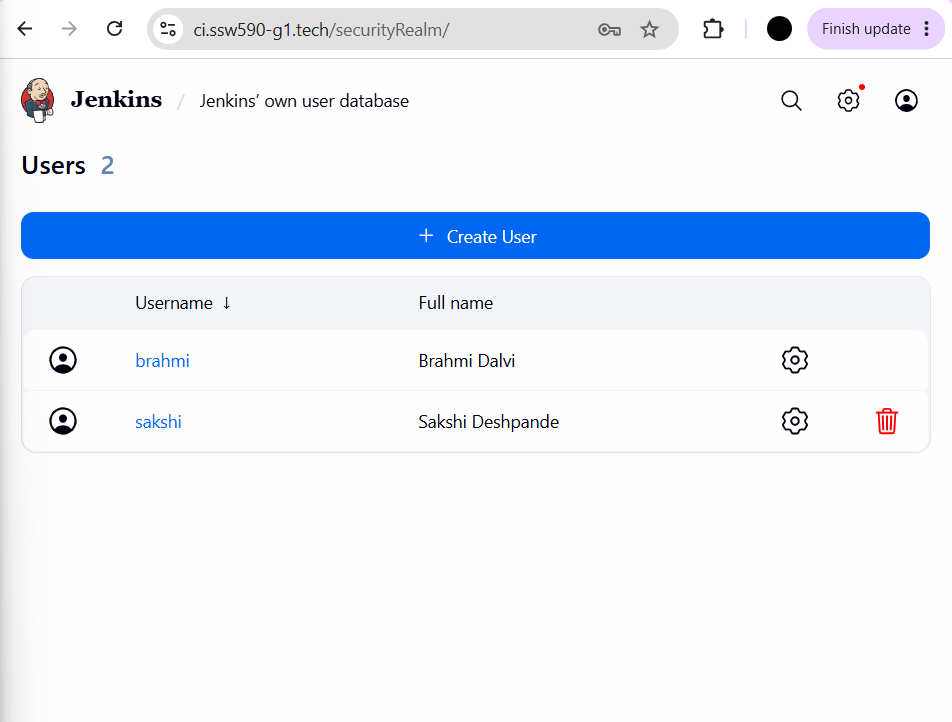
\includegraphics[width=0.75\linewidth]{evidence/79-jenkins-users-brahmi-sakshi-own-user-database-2026-11-02.png}
\caption{Jenkins Users page, November 2, 2026: two named accounts, \texttt{brahmi} and \texttt{sakshi}.}
\label{Fig:E79}
\end{figure}

\begin{figure}[htbp]
\centering
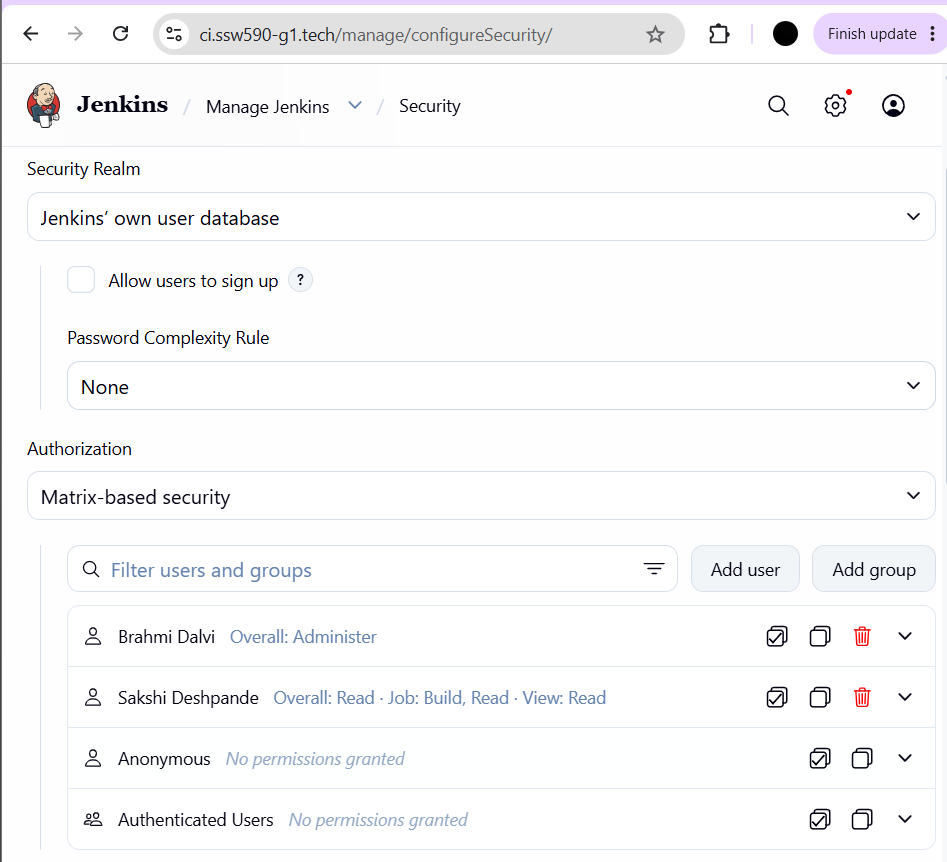
\includegraphics[width=0.85\linewidth]{evidence/80-jenkins-security-matrix-brahmi-administer-sakshi-read-build-anonymous-none-2026-11-02.png}
\caption{Manage Jenkins, Security, November 2, 2026: sign-up off; matrix authorization with Brahmi = Administer, Sakshi = Read and Build, Anonymous and Authenticated Users = no permissions.}
\label{Fig:E80}
\end{figure}

\paragraph{Firewall and ports.} No AWS rule was added for Jenkins. The security group still admits only 443 and 80 from
anyone and SSH (22) from the administrator's address, has no IPv6 rule, and has no rule for 8080, 50000, or 3000; the
Jenkins container publishes nothing, and Caddy's 80 and 443 are the only published ports. No host firewall such as
\texttt{ufw} is used, because Docker-published ports bypass it \cite{DockerFirewall}; the security group is the boundary and
exposure was tested from outside.

\begin{tabularx}{\linewidth}{L{3.2cm}L{3.3cm}L{3.4cm}Y}
\caption{External tests, November 2, 2026, expected versus actual\label{Table:JenkinsExternal}}\\
\toprule \textbf{Target} & \textbf{Expected} & \textbf{Actual} & \textbf{Source}\\ \midrule
\endfirsthead
\toprule \textbf{Target} & \textbf{Expected} & \textbf{Actual} & \textbf{Source}\\ \midrule
\endhead \bottomrule \endlastfoot
HTTPS 443, \texttt{/login} & opens for anyone & opens (HTTP 200; phone on mobile data) & \FigRef{76}, \ListRef{75}\\
HTTPS 443, \texttt{/} & plain Forbidden for non-team addresses & Forbidden on the phone & \FigRef{76}, right image\\
HTTP 80 & redirect to HTTPS & 308 to \texttt{https://ci.ssw590-g1.tech/} & \ListRef{75}\\
Raw port 8080 & unreachable & closed/filtered & \ListRef{103}, \ListRef{73}\\
Agent port 50000 & unreachable & closed/filtered & \ListRef{103}\\
Gitea backend 3000 & unreachable & closed/filtered & \ListRef{103}\\
IPv6 & not applicable & no AAAA record, no IPv6 rule & \ListRef{103}\\
\end{tabularx}
The 8080/50000/3000 probes ran from the administrator's computer; because the security group has no rule for those ports for
any address, a probe from another network cannot behave differently. The outsider's view of 443 was tested from the phone.
IPv6 is not enabled, so the equivalent IPv6 checks are not applicable; the deployment is IPv4 only.

\begin{longlisting}
\inputminted[fontsize=\scriptsize]{text}{evidence/103-security-group-port-probes-and-dns-for-jenkins-2026-11-02.txt}
\caption{Security group rules (administrator address redacted), external port probes, and DNS records, November 2, 2026 (real output).}
\label{Listing:E103}
\end{longlisting}

% ======================================================================
% Region: jenkTrigger (single owner; edit only your own region)
\subsection{Gitea trigger and traceability (15 points)}
\label{Section:jenkTrigger}
\textbf{Owner:} BD. \textbf{Status:} a webhook-started build observed after one corrected attempt \StatusPass.

\begin{figure}[htbp]
\centering
\resizebox{\linewidth}{!}{% Owner: BD. UML-style deployment diagram of the Group 1 Gitea + Jenkins integration on one AWS EC2 instance.
% Adapted from the course manual's Figure 4.2. Included by devopsJenkins.tex (jenkTrigger region). Only the tikzpicture lives here.
\begin{tikzpicture}[
  font=\footnotesize, >={Stealth[length=2.2mm]},
  node/.style={draw, rounded corners=2pt, fill=devopsLightBlue, align=center, minimum height=1.0cm, inner sep=3pt},
  who/.style={draw, rounded corners=2pt, fill=white, align=center, minimum height=0.9cm, minimum width=2.9cm, inner sep=3pt},
  store/.style={draw, fill=white, align=center, minimum height=0.8cm, inner sep=3pt},
  pub/.style={->, thick, devopsGreen},
  priv/.style={->, thick, devopsGray, dashed},
  lbl/.style={font=\scriptsize, align=center, fill=white, inner sep=1pt}]
  % browsers
  \node[who] (team) at (0,2.1) {Team browser\\(team address)};
  \node[who] (out) at (0,-0.2) {Any other browser\\(login page only)};
  % firewall
  \node[node, minimum height=3.6cm, minimum width=2.4cm] (sg) at (4.2,0.95) {AWS\\security group\\443, 80,\\22 (admin)};
  % EC2 box
  \draw[dashed, rounded corners=3pt] (6.3,-2.7) rectangle (18.6,4.95);
  \node[anchor=north west, font=\footnotesize\bfseries] at (6.4,4.9) {AWS EC2 instance (Docker network \texttt{gitea\_web})};
  % containers
  \node[node, minimum width=2.7cm] (caddy) at (8.1,0.95) {Caddy\\(TLS proxy)\\ports 443 and 80\\are the only ones\\published};
  \node[node, minimum width=4.6cm] (jenkins) at (15.4,2.2) {Jenkins controller 2.580.2\\\textbf{checkout and tests run here}\\(controller executor, python3)};
  \node[node, minimum width=4.6cm] (gitea) at (15.4,-1.3) {Gitea 1.27.3\\repositories, webhook,\\commit statuses};
  \node[store, minimum width=3.0cm] (jhome) at (15.4,4.0) {\texttt{jenkins\_home} volume};
  % browsers to firewall to Caddy
  \draw[pub] (team.east) -- node[lbl, above] {HTTPS 443} (sg.west |- team.east);
  \draw[pub] (out.east) -- node[lbl, above] {HTTPS 443} (sg.west |- out.east);
  \draw[pub] (sg.east |- caddy.west) -- (caddy.west);
  % Caddy to Jenkins and Gitea
  \draw[pub] (caddy.north east) |- node[lbl, pos=0.62, above] {\texttt{ci.} host: team address\\everything, others\\\texttt{/login} only} (jenkins.west);
  \draw[pub] (caddy.south east) |- node[lbl, pos=0.62, below] {\texttt{git.} host} (gitea.west);
  % private paths between Gitea and Jenkins, and the volume
  \draw[priv] ([xshift=-1.2cm]gitea.north) -- node[lbl, left] {webhook (POST),\\private network:\\\texttt{http://jenkins:8080/}\\\texttt{gitea-webhook/post}} ([xshift=-1.2cm]jenkins.south);
  \draw[priv] ([xshift=1.2cm]jenkins.south) -- node[lbl, right] {checkout and status\\(HTTPS to the\\public name)} ([xshift=1.2cm]gitea.north);
  \draw[thick] (jhome.south) -- (jenkins.north);
\end{tikzpicture}
}
\caption{UML-style deployment diagram of the actual browser and webhook paths on one EC2 instance, adapted from the course manual's Figure~4.2. Solid green: browser and proxy paths. Dashed grey: private paths between Gitea and Jenkins. Builds run on the Jenkins controller executor \cite{DosManual,JenkinsGiteaPlugin}.}
\label{Figure:JenkinsDeployment}
\end{figure}

\begin{tabularx}{\linewidth}{L{3.6cm}Y}
\caption{Gitea to Jenkins integration\label{Table:JenkinsIntegration}}\\
\toprule \textbf{Item} & \textbf{Value}\\ \midrule
\endfirsthead
\toprule \textbf{Item} & \textbf{Value}\\ \midrule
\endhead \bottomrule \endlastfoot
Repository & \href{\GiteaURL/group1-startup/twintrack}{\texttt{group1-startup/twintrack}} (public)\\
Integration identity & A dedicated Gitea user \texttt{jenkins-bot} with \emph{Write} on \texttt{twintrack} only (\FigRef{82}); its token is stored only in the Jenkins credential \texttt{gitea-jenkins-bot} (\FigRef{83}). The scopes were chosen narrow (user and organization read, repository write); the exact scope list was not captured as evidence\\
Jenkins job & Multibranch Pipeline \texttt{twintrack} (Gitea plugin), which found the \texttt{Jenkinsfile} in pull request \#10 and scheduled build \texttt{PR-10} (\FigRef{84})\\
Webhook & Repository level: \texttt{http://jenkins:8080/gitea-webhook/post} on the private Docker network, POST with JSON; events \emph{Push}, \emph{Pull Request}, and \emph{Pull Request Synchronized} (the last was added after a failed attempt, see below); no webhook secret (\FigRef{86}, \FigRef{87})\\
Gitea setting & \texttt{[webhook] ALLOWED\_HOST\_LIST = jenkins}: Gitea blocks webhooks to private addresses by default \cite{GiteaConfig,GiteaWebhooks}; only the host name \texttt{jenkins} is allowed (\ListRef{81})\\
Where code runs & Checkout and tests run in a workspace inside the Jenkins container (controller executor). Jenkins fetches the code from \texttt{https://git.ssw590-g1.tech} (the public name, through Caddy) and posts statuses back to the same API\\
Status reported & Context \textbf{\texttt{twintrack/pipeline/pr-main}}, posted as \texttt{jenkins-bot}: pending, then success or failure (\ListRef{85})\\
\end{tabularx}

\begin{figure}[htbp]
\centering
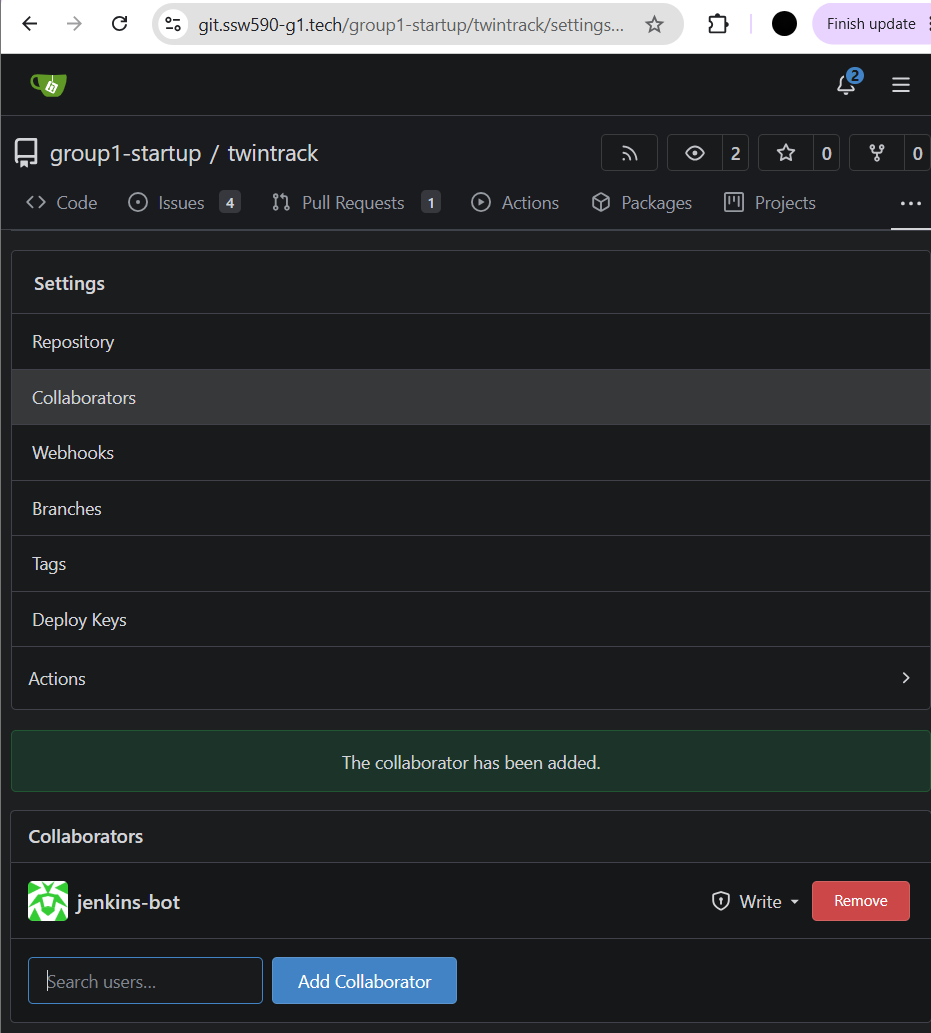
\includegraphics[width=0.8\linewidth]{evidence/82-gitea-twintrack-collaborator-jenkins-bot-write-2026-11-02.png}
\caption{\texttt{twintrack} Settings, Collaborators, November 2, 2026: \texttt{jenkins-bot} added with Write.}
\label{Fig:E82}
\end{figure}

\begin{figure}[htbp]
\centering
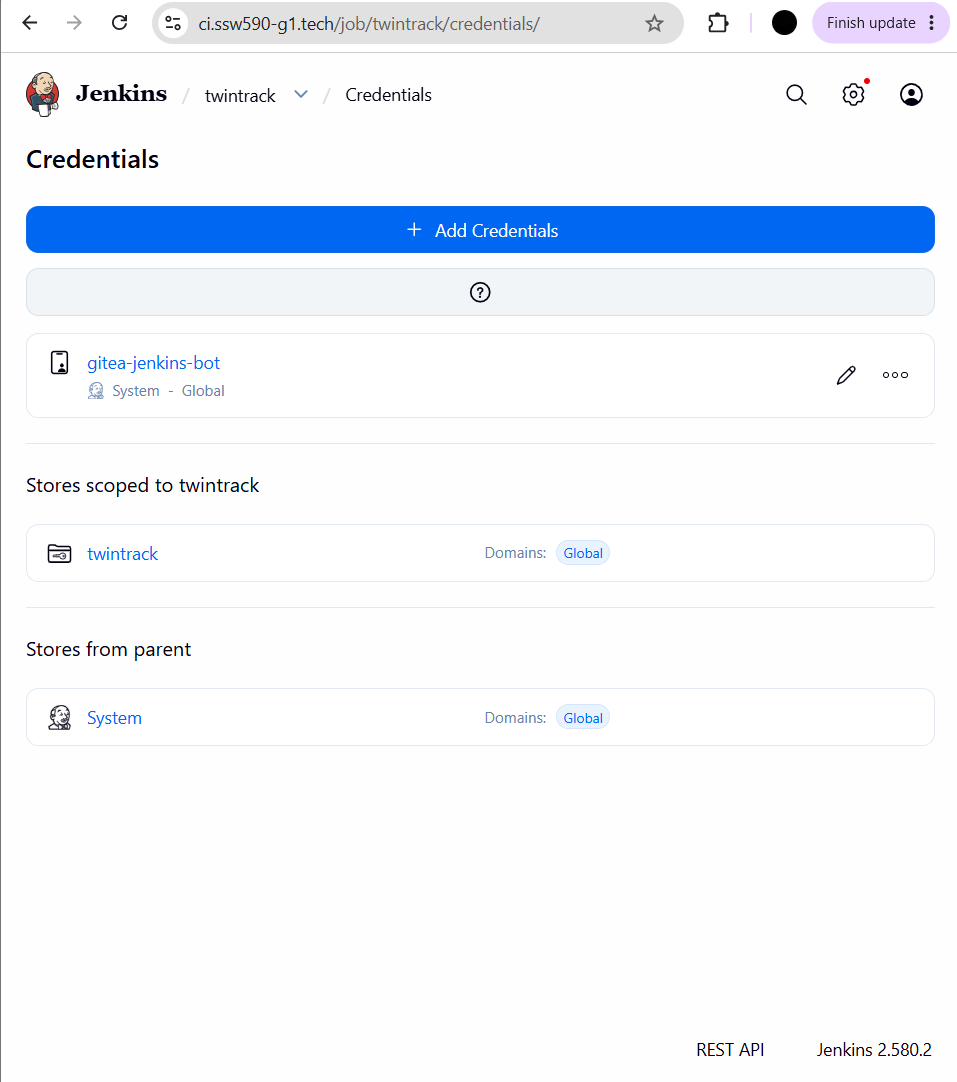
\includegraphics[width=0.7\linewidth]{evidence/83-jenkins-credentials-gitea-jenkins-bot-secret-hidden-2026-11-02.png}
\caption{Jenkins Credentials, November 2, 2026: \texttt{gitea-jenkins-bot} (System, Global). The token is stored in Jenkins and is not displayed.}
\label{Fig:E83}
\end{figure}

\begin{figure}[htbp]
\centering
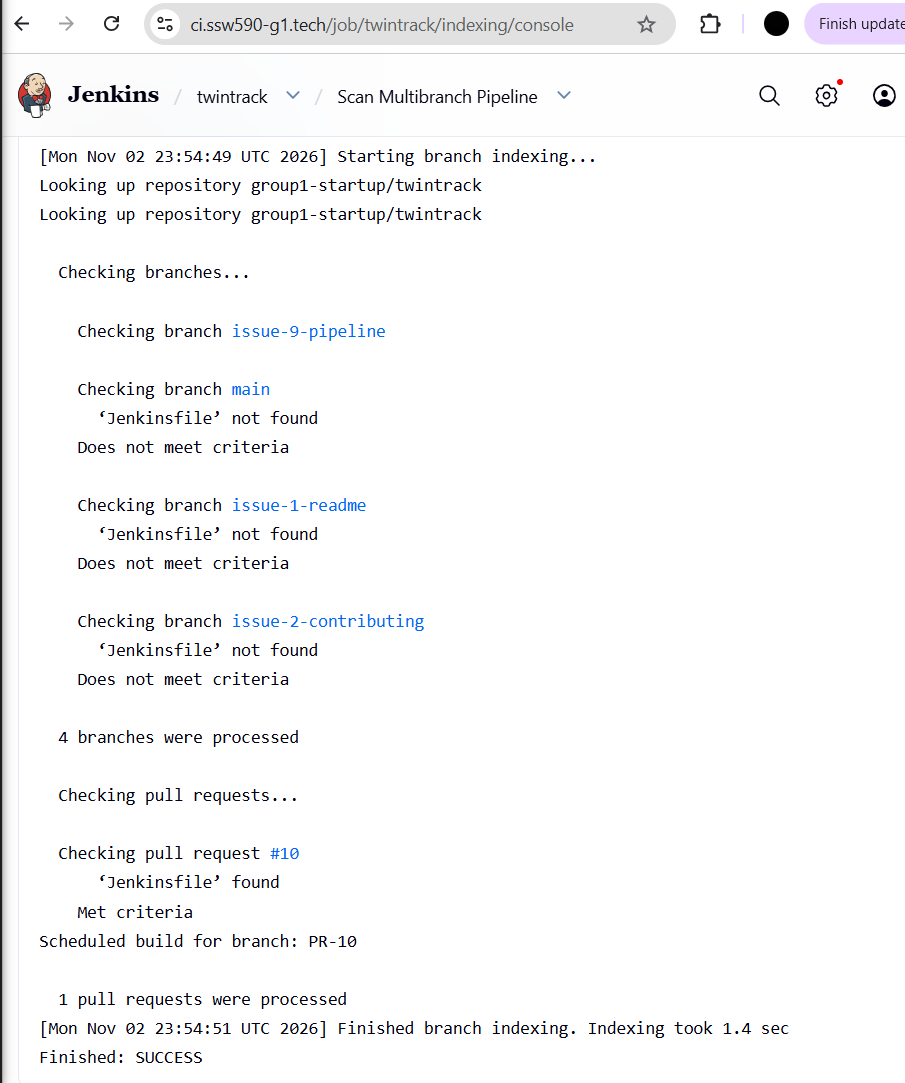
\includegraphics[width=0.8\linewidth]{evidence/84-jenkins-multibranch-scan-console-pr10-scheduled-2026-11-02.png}
\caption{Multibranch scan of \texttt{group1-startup/twintrack}, November 2, 2026 (23:54 UTC): branches without a \texttt{Jenkinsfile} do not meet the criteria; pull request \#10 does, and ``Scheduled build for branch: PR-10''.}
\label{Fig:E84}
\end{figure}

\paragraph{Delivery result and the linked Jenkins run.} A \emph{Test Push Event} reached
\texttt{http://jenkins:8080/gitea-webhook/post} and returned HTTP~200 (\FigRef{87}). The first build that
the webhook itself started is Jenkins build \#3 (cause \texttt{BranchEventCause}, console line ``Pull request \#10
event'') for commit \texttt{d5e5c64}, which passed in about 5 seconds; Gitea holds the matching status for the same commit
(\ListRef{94}). Builds \#4 and \#5 (commits \texttt{86ee9fc} and \texttt{92c121d}) were also started by the webhook
(\ListRef{96}, \ListRef{99}). The commit ID is therefore the same in Gitea, in the Jenkins log, and in the status.

\begin{figure}[htbp]
\centering
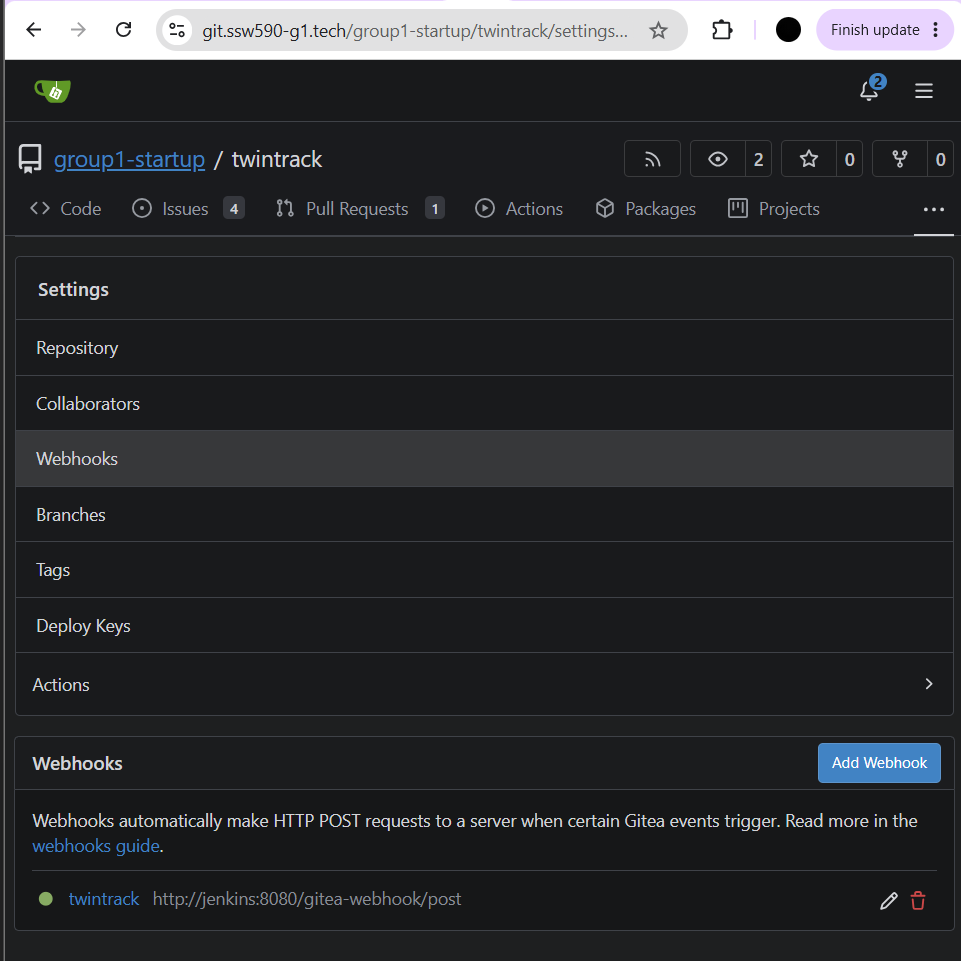
\includegraphics[width=0.75\linewidth]{evidence/86-gitea-twintrack-repository-webhook-to-jenkins-green-2026-11-02.png}
\caption{\texttt{twintrack} Settings, Webhooks (repository level), November 2, 2026: the webhook to \texttt{http://jenkins:8080/gitea-webhook/post}, status dot green.}
\label{Fig:E86}
\end{figure}

\begin{figure}[htbp]
\centering
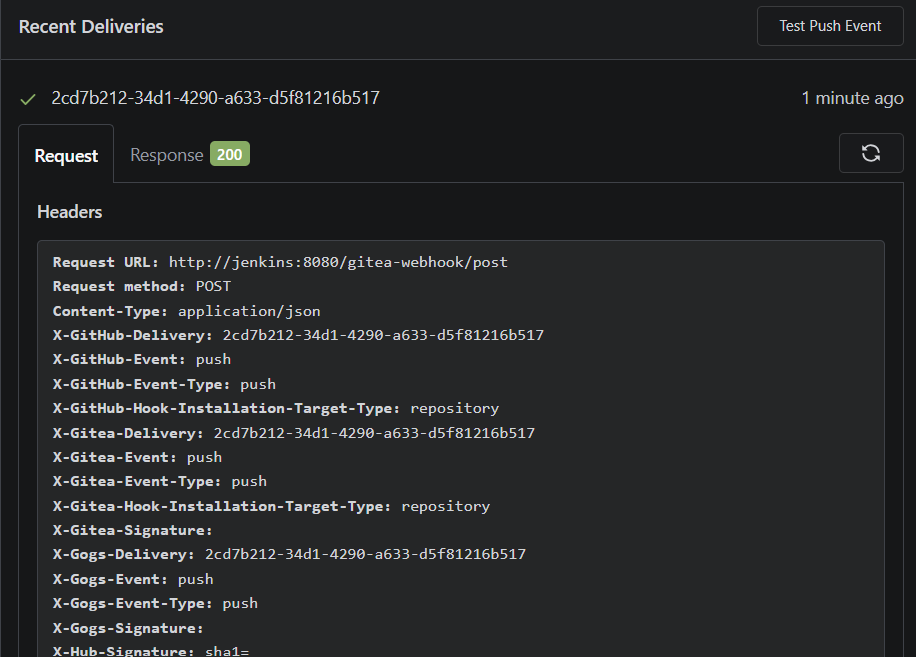
\includegraphics[width=0.85\linewidth]{evidence/87-gitea-webhook-delivery-test-push-response-200-2026-11-02.png}
\caption{Recent Deliveries of the webhook: a Test Push Event to the private address, POST \texttt{application/json}, response 200. The signature headers are empty because no webhook secret is configured.}
\label{Fig:E87}
\end{figure}

\begin{longlisting}
\inputminted[fontsize=\scriptsize]{text}{evidence/94-jenkins-pr10-build-3-webhook-triggered-success-and-gitea-status-2026-11-02.txt}
\caption{Build \#3, the first build started by the webhook: cause, console, and Gitea statuses for commit \texttt{d5e5c64}, November 2, 2026 (real output).}
\label{Listing:E94}
\end{longlisting}

\paragraph{A failed delivery, diagnosed and corrected.} The first webhook attempt did not start builds for new
commits, and the cause was found in two steps. (1) BD first created the webhook in her \emph{personal} account
settings (the page said it fires for ``all repositories that you own''), but \texttt{twintrack} belongs to the organization,
so it never fired; it was recreated on the repository. (2) Even then, a real push to the pull request branch reached Jenkins
(its \emph{Multibranch Pipeline Events} page lists three push events processed in under a second each, \ListRef{93}) but
no build was scheduled, because the webhook did not have the \emph{Pull Request Synchronized} event ticked
(\FigRef{92}): a plain push event only re-checks branches, and the branch behind a pull request is skipped, so only the
pull-request event tells Jenkins to rebuild the new head commit. Ticking that event fixed it, proven by build \#3. In the
meantime build \#2 had been started by hand and the repair commit \texttt{7d7848f} was never built.
\textbf{Operator steps for a failed delivery:} open the webhook's \emph{Recent Deliveries} in Gitea (did it send, to which URL,
which response?); open \emph{Multibranch Pipeline Events} in Jenkins (was the event received, and what did it do?); check the
events ticked in the webhook; check the allowed-host setting and that the URL uses the container name \texttt{jenkins}; then
use \emph{Scan Repository Now} as a manual fallback.

\begin{figure}[htbp]
\centering
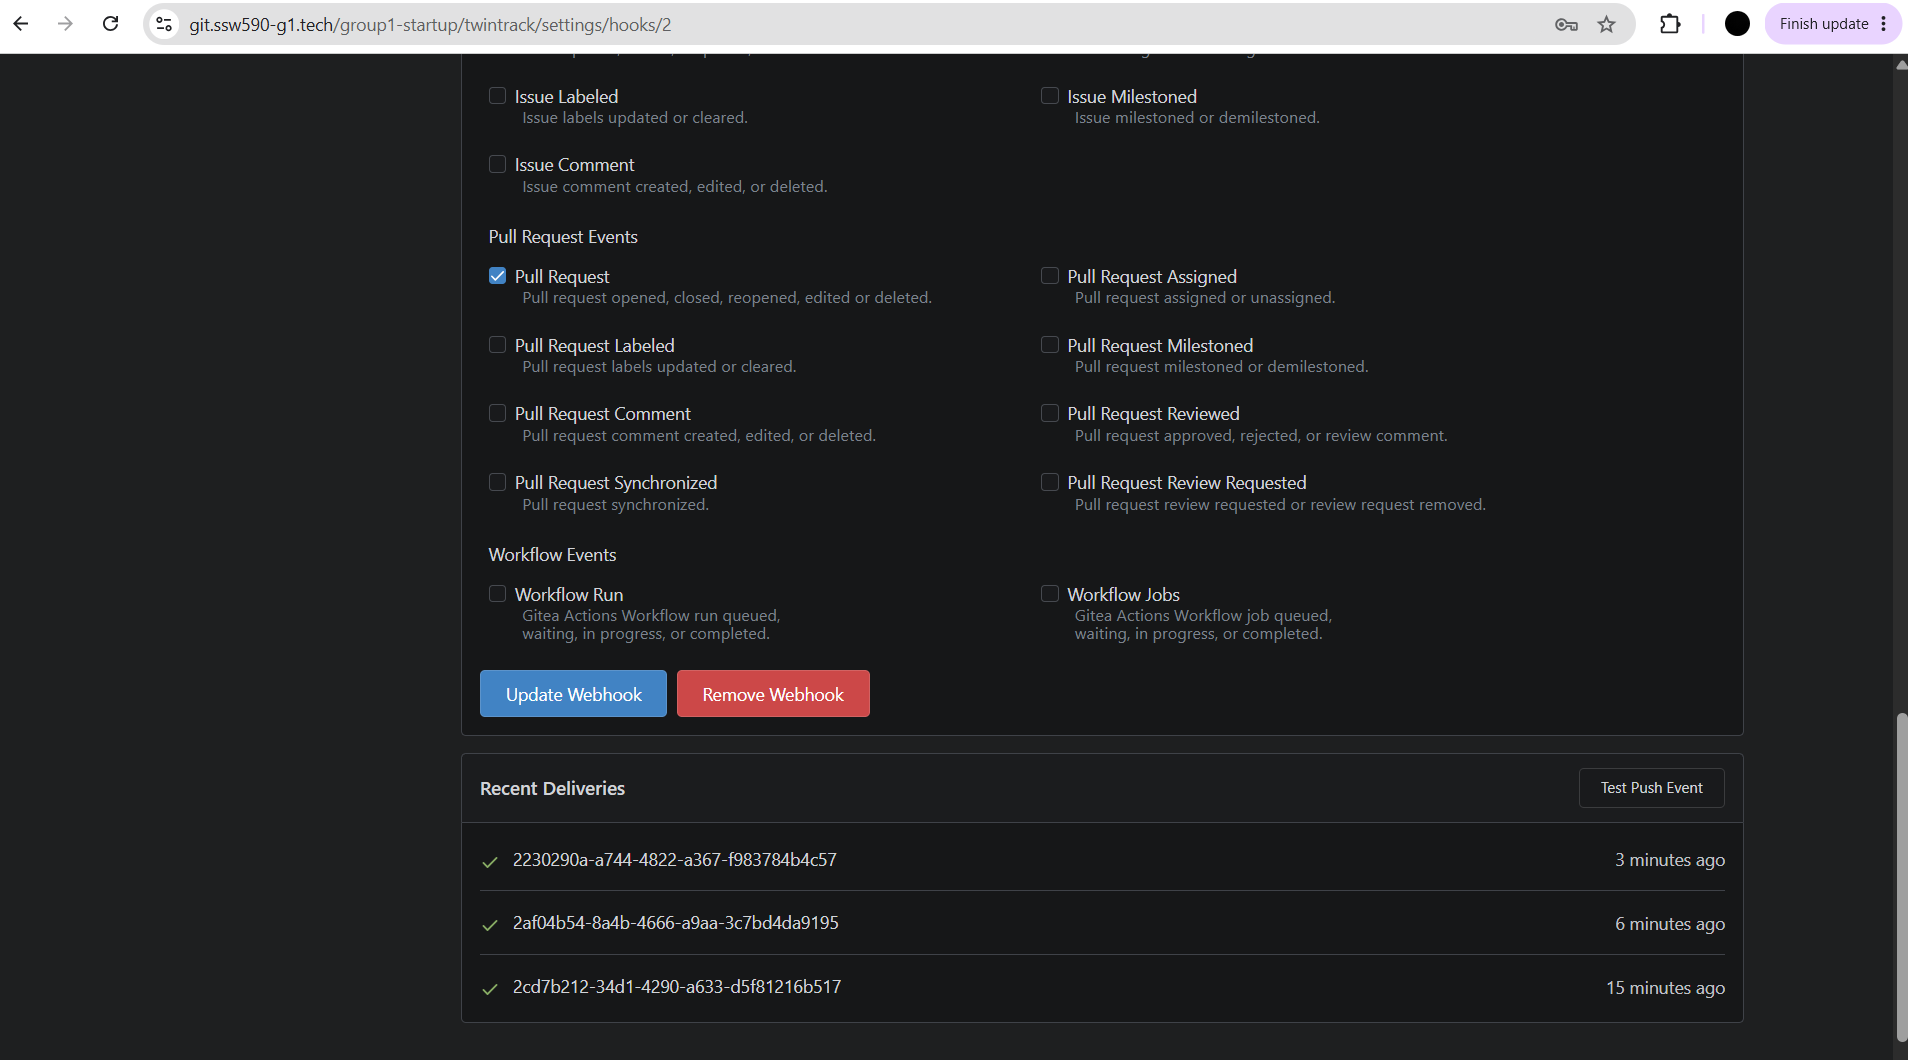
\includegraphics[width=\linewidth]{evidence/92-gitea-webhook-trigger-events-pull-request-synchronized-unticked-2026-11-02.png}
\caption{The webhook's events before the fix, November 2, 2026: \emph{Pull Request} is ticked and \emph{Pull Request Synchronized} is not; the three deliveries below all succeeded.}
\label{Fig:E92}
\end{figure}

\begin{longlisting}
\inputminted[fontsize=\scriptsize]{text}{evidence/93-jenkins-multibranch-pipeline-events-log-push-events-no-build-2026-11-02.txt}
\caption{Jenkins \emph{Multibranch Pipeline Events} (copied by Brahmi): push events received and processed, but no build scheduled (real output).}
\label{Listing:E93}
\end{longlisting}

\begin{longlisting}
\inputminted[fontsize=\scriptsize]{text}{evidence/81-gitea-webhook-allowed-host-jenkins-recreate-2026-11-02.txt}
\caption{Allowing the webhook host \texttt{jenkins} in Gitea: compose change, only Gitea recreated (healthy after 37 seconds), setting confirmed, data intact, November 2, 2026 (real output).}
\label{Listing:E81}
\end{longlisting}

% ======================================================================
% Region: jenkPipeline (single owner; edit only your own region)
\subsection{Versioned pipeline and tests (15 points)}
\label{Section:jenkPipeline}
\index{Jenkinsfile}
\index{pipeline}
\textbf{Owner:} SD. \textbf{Status:} drafted by BD from the real runs; every statement checked by SD on
November 3, 2026 against Gitea's records, the Jenkins evidence, and a clean local run \StatusPass.

The application is the course's optional minimal Python example (manual Chapter~4, step~4), committed to
\texttt{twintrack} through the issue-linked pull request \#10 (issue \#9): \texttt{pricing.py}, \texttt{tests/test\_pricing.py}, and a
\texttt{Jenkinsfile} at the repository root. The files are linked at the commit that Jenkins tested last
(\href{\GiteaURL/group1-startup/twintrack/src/commit/92c121dec9da4c51e5080b198e82be7c405df799/Jenkinsfile}{\texttt{Jenkinsfile}},
\href{\GiteaURL/group1-startup/twintrack/src/commit/92c121dec9da4c51e5080b198e82be7c405df799/pricing.py}{\texttt{pricing.py}}).

\begin{longlisting}
\inputminted[fontsize=\scriptsize]{groovy}{config/twintrack/Jenkinsfile}
\caption{The declarative \texttt{Jenkinsfile}: Checkout, Syntax check, Test.}
\label{Listing:JenkinsFile}
\end{longlisting}

\begin{longlisting}
\inputminted[fontsize=\scriptsize]{python}{config/twintrack/pricing.py}
\inputminted[fontsize=\scriptsize]{python}{config/twintrack/tests/test_pricing.py}
\caption{\texttt{pricing.py} and \texttt{tests/test\_pricing.py}.}
\label{Listing:JenkinsApp}
\end{longlisting}

\begin{tabularx}{\linewidth}{L{3.2cm}Y}
\caption{Pipeline stages\label{Table:JenkinsStages}}\\
\toprule \textbf{Stage} & \textbf{What it does and expected result}\\ \midrule
\endfirsthead
\toprule \textbf{Stage} & \textbf{What it does and expected result}\\ \midrule
\endhead \bottomrule \endlastfoot
Checkout & \texttt{checkout scm} fetches the pull request head, merged with \texttt{main}, from Gitea; the log names the exact revision\\
Syntax check (build/lint) & \texttt{python3 -m py\_compile pricing.py}: fails on any syntax error; silent success otherwise\\
Test & \texttt{python3 -m unittest discover -s tests -v}: two tests; the stage fails if any test fails, with the assertion in the log\\
\end{tabularx}

\paragraph{Dependencies and clean run.} The only dependency is Python~3 on the executor (3.13.5, installed in the image by
\texttt{apt}); there are no packages from the internet. A clean run is reproduced on any computer with Python~3: clone the repository, then run
\texttt{python3 -m py\_compile pricing.py} and \texttt{python3 -m unittest discover -s tests -v} in it. This was done before the
first push (\ListRef{70}) and again by SD on November 3, 2026, in a fresh clone of the merged \texttt{main} (commit \texttt{a0094a8},
\ListRef{108}): syntax OK, two tests \texttt{ok}, exit code~0, the same result as Jenkins.

\paragraph{Run view and stage results.} The Jenkins Pipeline Stage View plugin is not installed, so there is no graphical stage
view; the distinct stage results are in the console log (\ListRef{85}): after the checkout, the \emph{Syntax check} stage runs
\texttt{py\_compile}, and the \emph{Test} stage prints the two tests as \texttt{ok}, followed by \texttt{Finished: SUCCESS}. The first
passing run tested commit \texttt{da16c9b} (build \#1); the log also shows what exactly is tested: Jenkins fetches the pull
request head and \texttt{main}, then reports ``Merging remotes/origin/main commit \texttt{0d0c3da} into PR head commit
\texttt{da16c9b}'', so a pull request build tests the result of the merge, not the branch alone. The Gitea statuses and the build
records are in the same listing. The failing
stage is visible in the failing builds (\ListRef{96}).

\begin{longlisting}
\inputminted[fontsize=\scriptsize]{text}{evidence/70-local-test-run-pricing-example-2026-10-29.txt}
\caption{Local run of the course example before the first pull request, October 29, 2026 (real output).}
\label{Listing:E70}
\end{longlisting}

\begin{longlisting}
\inputminted[fontsize=\scriptsize]{text}{evidence/85-jenkins-pr10-build-1-console-and-gitea-commit-status-2026-11-02.txt}
\caption{Build \#1 of \texttt{PR-10} (commit \texttt{da16c9b}): console, stage commands, and the Gitea statuses (real output; console annotation blobs removed).}
\label{Listing:E85}
\end{longlisting}

\begin{longlisting}
\inputminted[fontsize=\scriptsize]{text}{evidence/108-clean-clone-test-run-main-a0094a8-sd-2026-11-03.txt}
\caption{Clean-run check by SD: fresh clone of \texttt{twintrack} at the merged commit \texttt{a0094a8}, the two pipeline commands, November 3, 2026 (real output).}
\label{Listing:E108}
\end{longlisting}

% ======================================================================
% Region: jenkGate (single owner; edit only your own region)
\subsection{Required merge gate (15 points)}
\label{Section:jenkGate}
\index{status check}
\index{merge gate}
\textbf{Owner:} SD. \textbf{Status:} drafted by BD from the real runs; checked by SD on November 3, 2026 against
Gitea's branch, status, and timeline records (\ListRef{107}) \StatusPass.

\paragraph{The rule.} The default branch \texttt{main} of \texttt{twintrack} is protected in Gitea: pushes go through pull
requests, \emph{one approving review} is required, and the \textbf{status check pattern
\texttt{twintrack/pipeline/pr-main}} is required \cite{GiteaProtectedBranches}. That is the exact context Jenkins reports; Gitea itself listed it
as ``Matched'' among the status checks found in the last week before the rule was saved (\FigRef{88}). A delivered webhook or a green page
inside Jenkins is not the gate: the gate is Gitea's own record of this status on the pull request's latest head commit.

\begin{figure}[htbp]
\centering
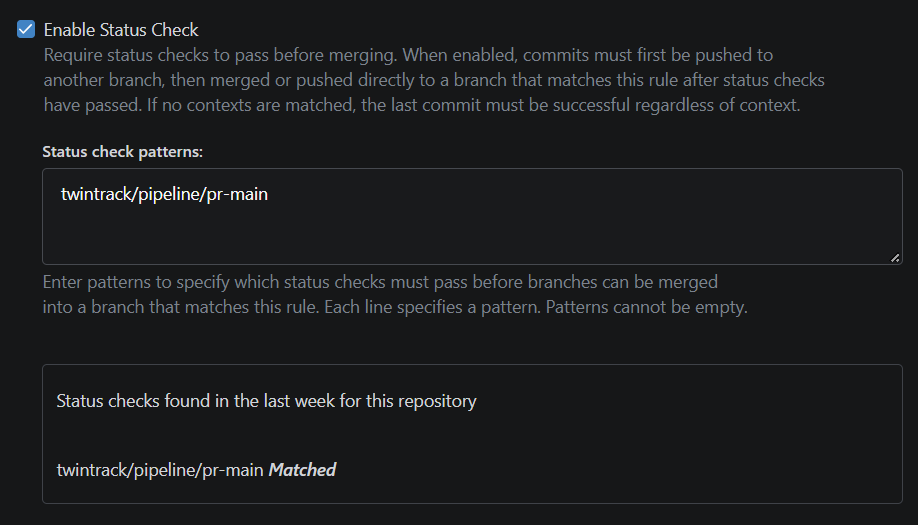
\includegraphics[width=0.85\linewidth]{evidence/88-gitea-twintrack-main-rule-status-check-pr-main-matched-2026-11-02.png}
\caption{Branch rule for \texttt{main}, November 2, 2026: \emph{Enable Status Check} ticked, pattern \texttt{twintrack/pipeline/pr-main}, shown as ``Matched''. Saved: Gitea's API reports \texttt{enable\_status\_check: true} with that context and one required approval.}
\label{Fig:E88}
\end{figure}

\paragraph{How the status reaches Gitea.} Jenkins' Gitea plugin posts it through Gitea's commit-status API with the token of
\texttt{jenkins-bot}: \emph{pending} when the build is queued and started, then \emph{success} or \emph{failure} when it ends; the console shows the
lines ``[Gitea] Notifying pull request build status'' for each step \cite{JenkinsGiteaPlugin,JenkinsGiteaChecks}. Gitea shows the result next to the commit
and uses the required context to allow or block the merge. Gitea's own records show the round trip for the two
merge-gate states (\ListRef{107}, UTC, November 3, 2026):

\begin{tabularx}{\linewidth}{L{2.0cm}L{1.8cm}L{2.6cm}L{2.6cm}Y}
\caption{From push to status in Gitea for the two merge-gate states\label{Table:JenkinsStatusTrip}}\\
\toprule \textbf{Head commit} & \textbf{Pushed} & \textbf{First \emph{pending}} & \textbf{Final status} & \textbf{Jenkins run}\\ \midrule
\endfirsthead
\toprule \textbf{Head commit} & \textbf{Pushed} & \textbf{First \emph{pending}} & \textbf{Final status} & \textbf{Jenkins run}\\ \midrule
\endhead \bottomrule \endlastfoot
\texttt{86ee9fc} & 00:30:22 & 00:30:24 & \textbf{failure} 00:30:38 & \href{https://ci.ssw590-g1.tech/job/twintrack/job/PR-10/4/}{\texttt{PR-10} \#4}\\
\texttt{92c121d} & 00:32:51 & 00:32:53 & \textbf{success} 00:33:18 & \href{https://ci.ssw590-g1.tech/job/twintrack/job/PR-10/5/}{\texttt{PR-10} \#5}\\
\end{tabularx}
The Jenkins run links need a Jenkins sign-in (Section~\ref{Section:jenkAccess}); the same run numbers are visible without
one as the target of each status in Gitea, and the pull request is public:
\href{\GiteaURL/group1-startup/twintrack/pulls/10}{pull request \#10}.

\paragraph{Failed check blocking the merge.} After the controlled failure (commit \texttt{86ee9fc}, November 2, 2026), the pull request page
reads \emph{Some required checks failed}: the required check \texttt{twintrack/pipeline/pr-main} shows ``There was a failure building this commit'',
and below it ``Some required checks were not successful'' and ``0 of 1 official approvals granted'' (\FigRef{97}). The failing commits
carry red crosses in the commit list, and Jenkins shows the job red (\FigRef{98}).

\begin{figure}[htbp]
\centering
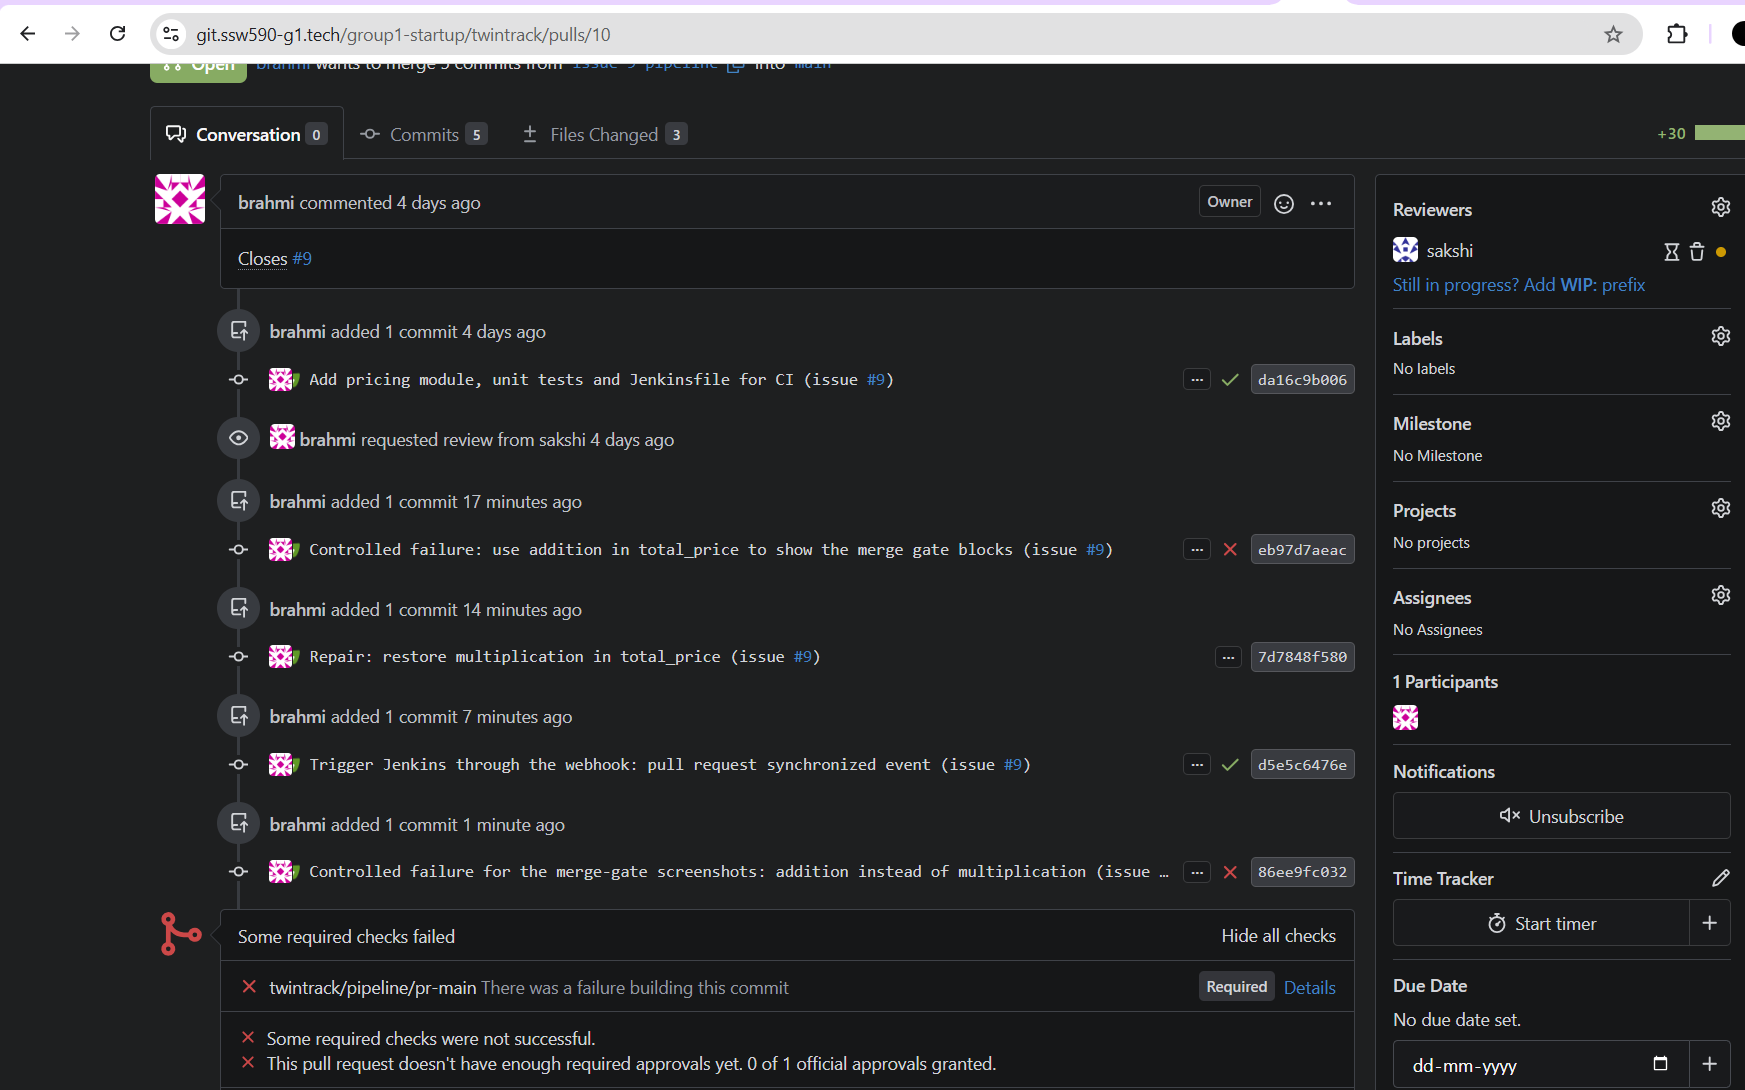
\includegraphics[width=\linewidth]{evidence/97-gitea-pr10-required-check-failed-merge-gate-commit-86ee9fc-2026-11-02.png}
\caption{\textbf{Failed check blocking the merge.} Pull request \#10, November 2, 2026, head commit \texttt{86ee9fc}, required check \texttt{twintrack/pipeline/pr-main} failed. The merge button area is below the cropped part of the page.}
\label{Fig:E97}
\end{figure}

\begin{figure}[htbp]
\centering
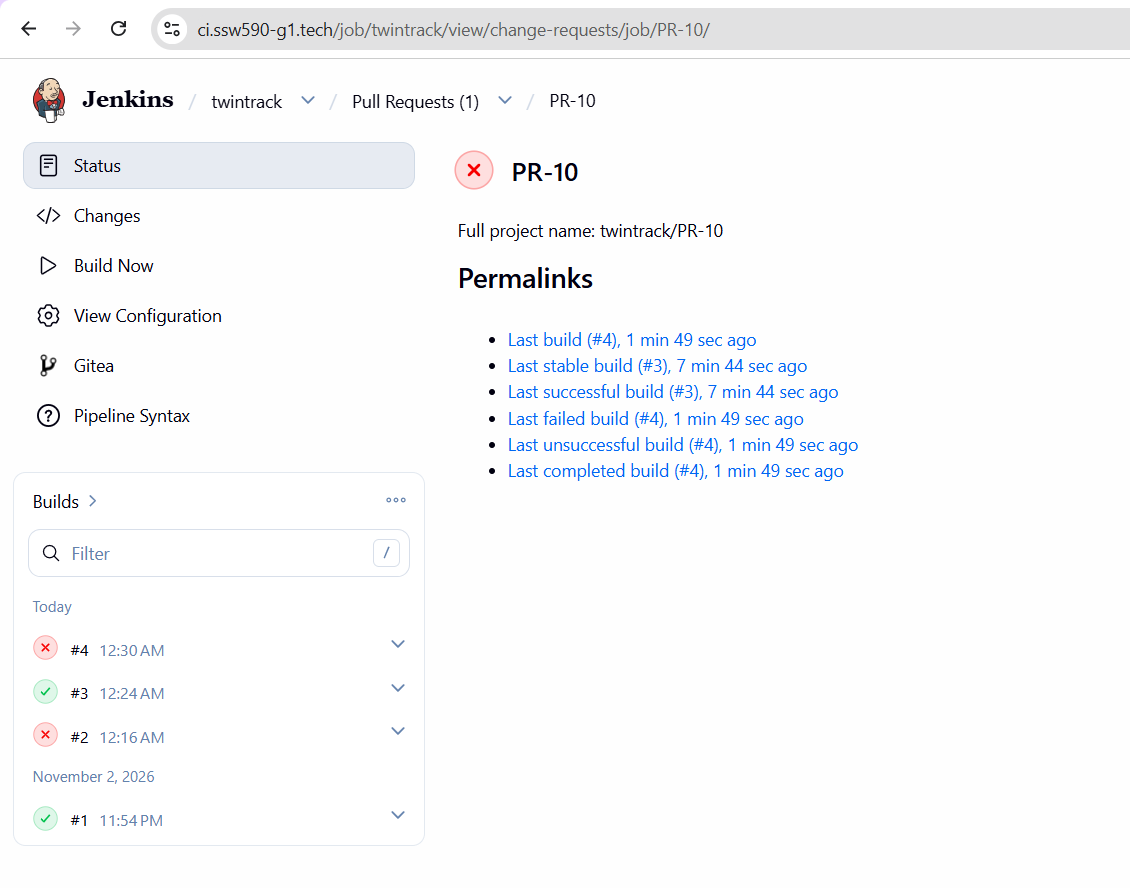
\includegraphics[width=0.8\linewidth]{evidence/98-jenkins-pr10-job-red-build-4-failed-build-3-last-stable-2026-11-02.png}
\caption{Jenkins job \texttt{PR-10} after the failing push, November 2, 2026: red, last build \#4 failed (12:30 AM UTC), last stable build \#3.}
\label{Fig:E98}
\end{figure}

\paragraph{Passing check after the repair.} After the repair (commit \texttt{92c121d}) the page reads \emph{All checks were successful}: the required check shows
``This commit looks good'' and the merge now waits only for the approving review (\FigRef{100}); Jenkins shows build \#5 green (\FigRef{101}).

\begin{figure}[htbp]
\centering
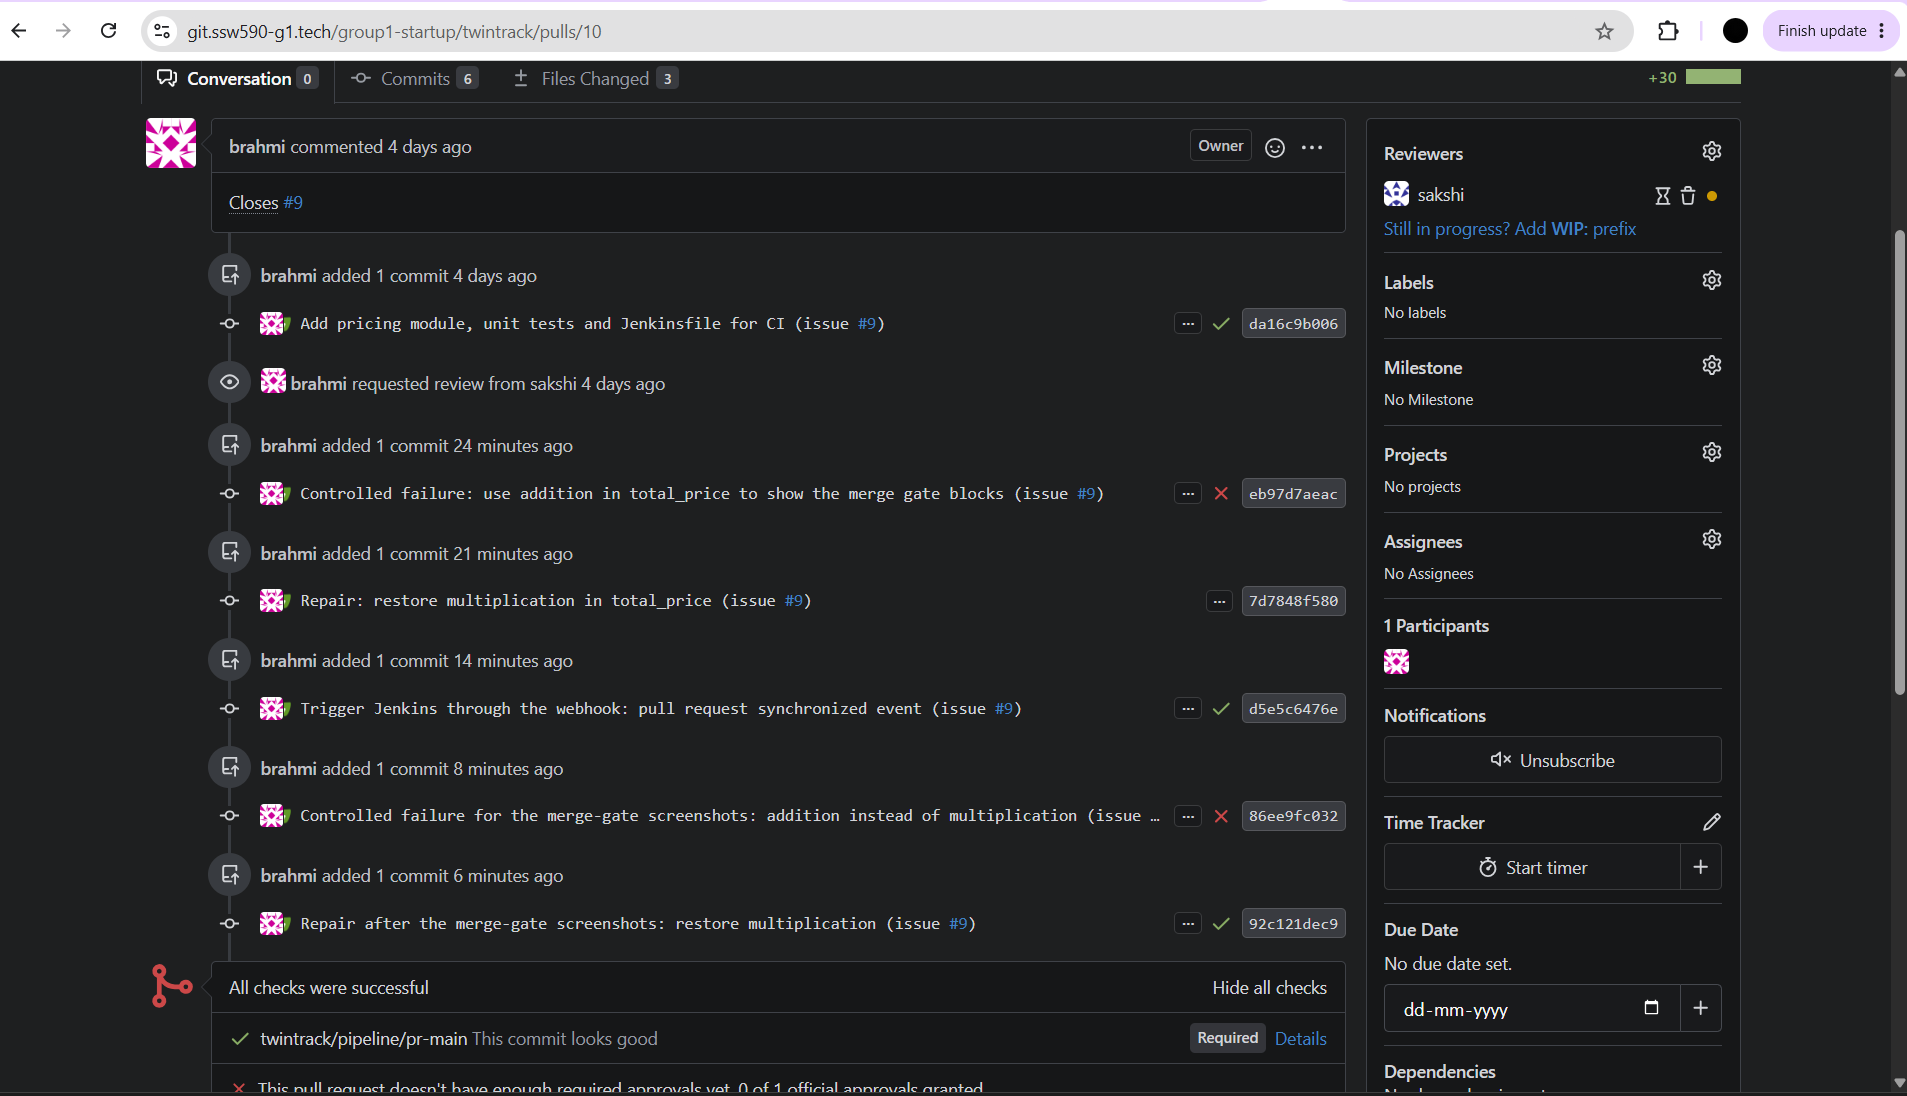
\includegraphics[width=\linewidth]{evidence/100-gitea-pr10-all-checks-successful-head-92c121d-6-commits-2026-11-02.png}
\caption{\textbf{Passing check after repair.} Pull request \#10, November 2, 2026, head commit \texttt{92c121d}, required check \texttt{twintrack/pipeline/pr-main} successful; the failed commits \texttt{eb97d7a} and \texttt{86ee9fc} are marked with red crosses; merge waiting for approval.}
\label{Fig:E100}
\end{figure}

\begin{figure}[htbp]
\centering
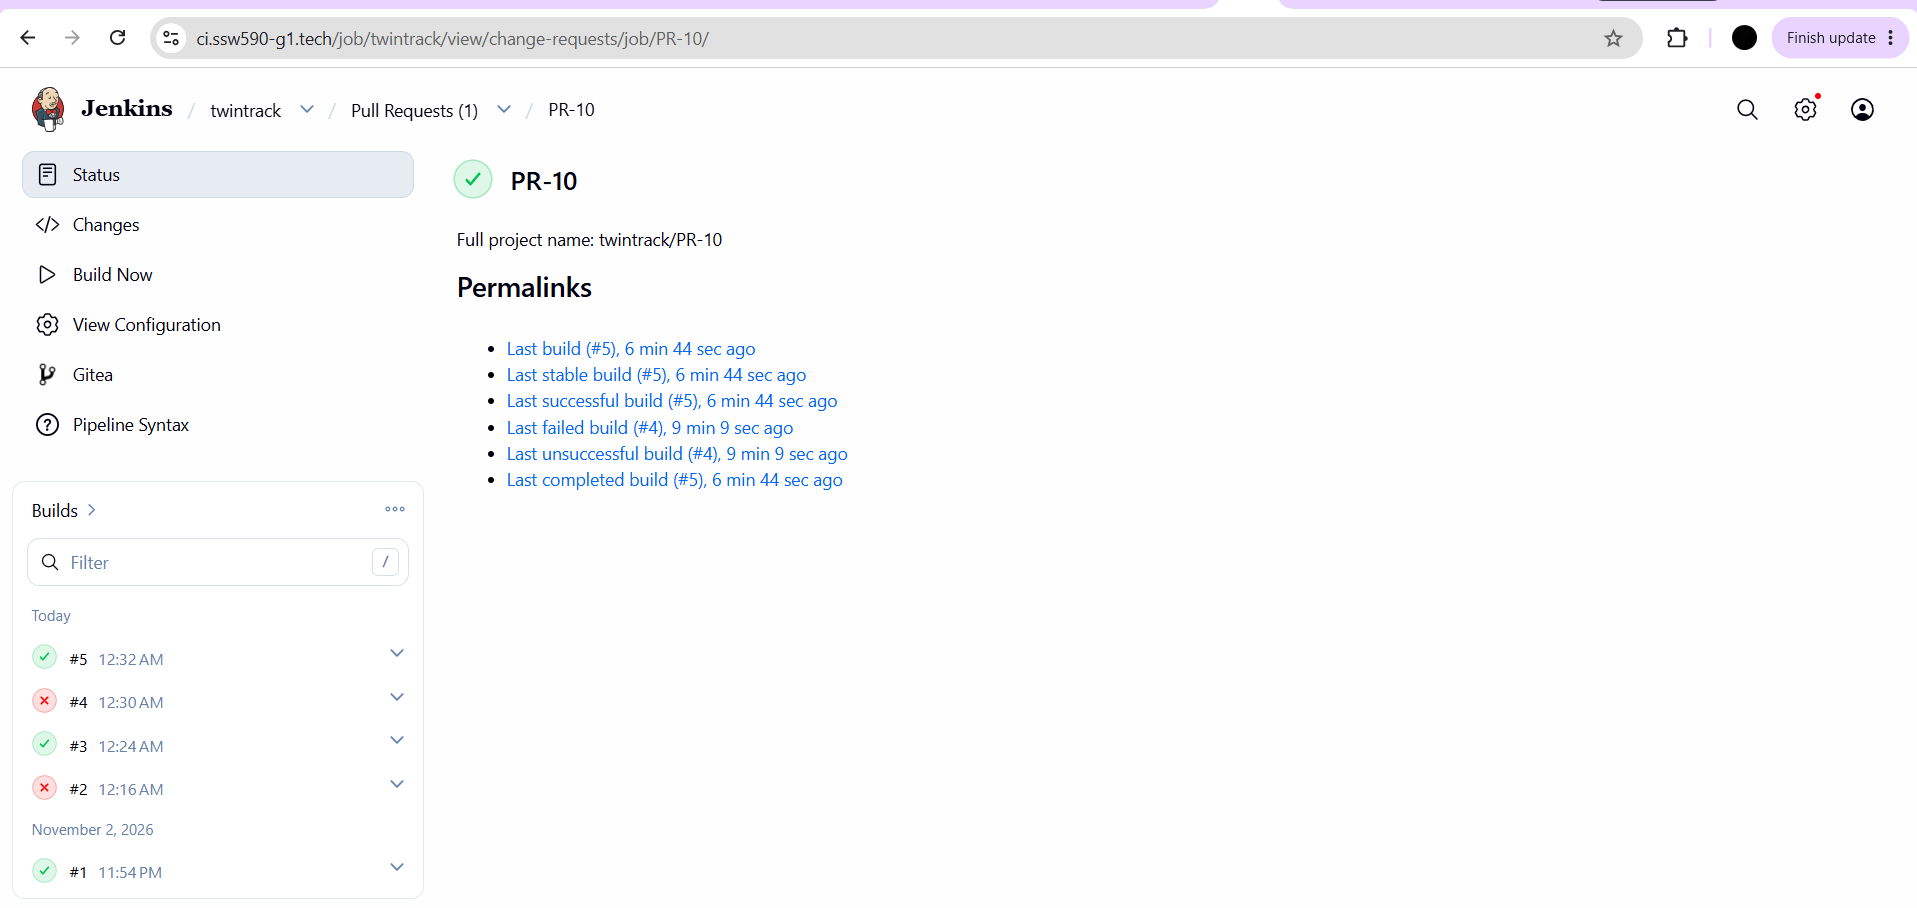
\includegraphics[width=0.8\linewidth]{evidence/101-jenkins-pr10-job-green-build-5-after-repair-history-2026-11-02.png}
\caption{Jenkins job \texttt{PR-10} after the repair, November 2, 2026: build \#5 green (12:32 AM UTC), build \#4 failed, history \#1 to \#5.}
\label{Fig:E101}
\end{figure}

\paragraph{A limit of this gate.} The repository owner is also a Gitea administrator, and an earlier screenshot of the pull request page showed
``As an administrator, you may still merge this pull request'' (\FigRef{90}). An owner could therefore override the rule; the team agreed not to, and Gitea's option
``Administrators must follow branch protection rules'', which removes that override \cite{GiteaProtectedBranches}, was not
enabled. No merge into \texttt{main} used the override: pull request \#10 was merged only after the check passed and SD approved
it (Section~\ref{Section:jenkFailure}).

\begin{figure}[htbp]
\centering
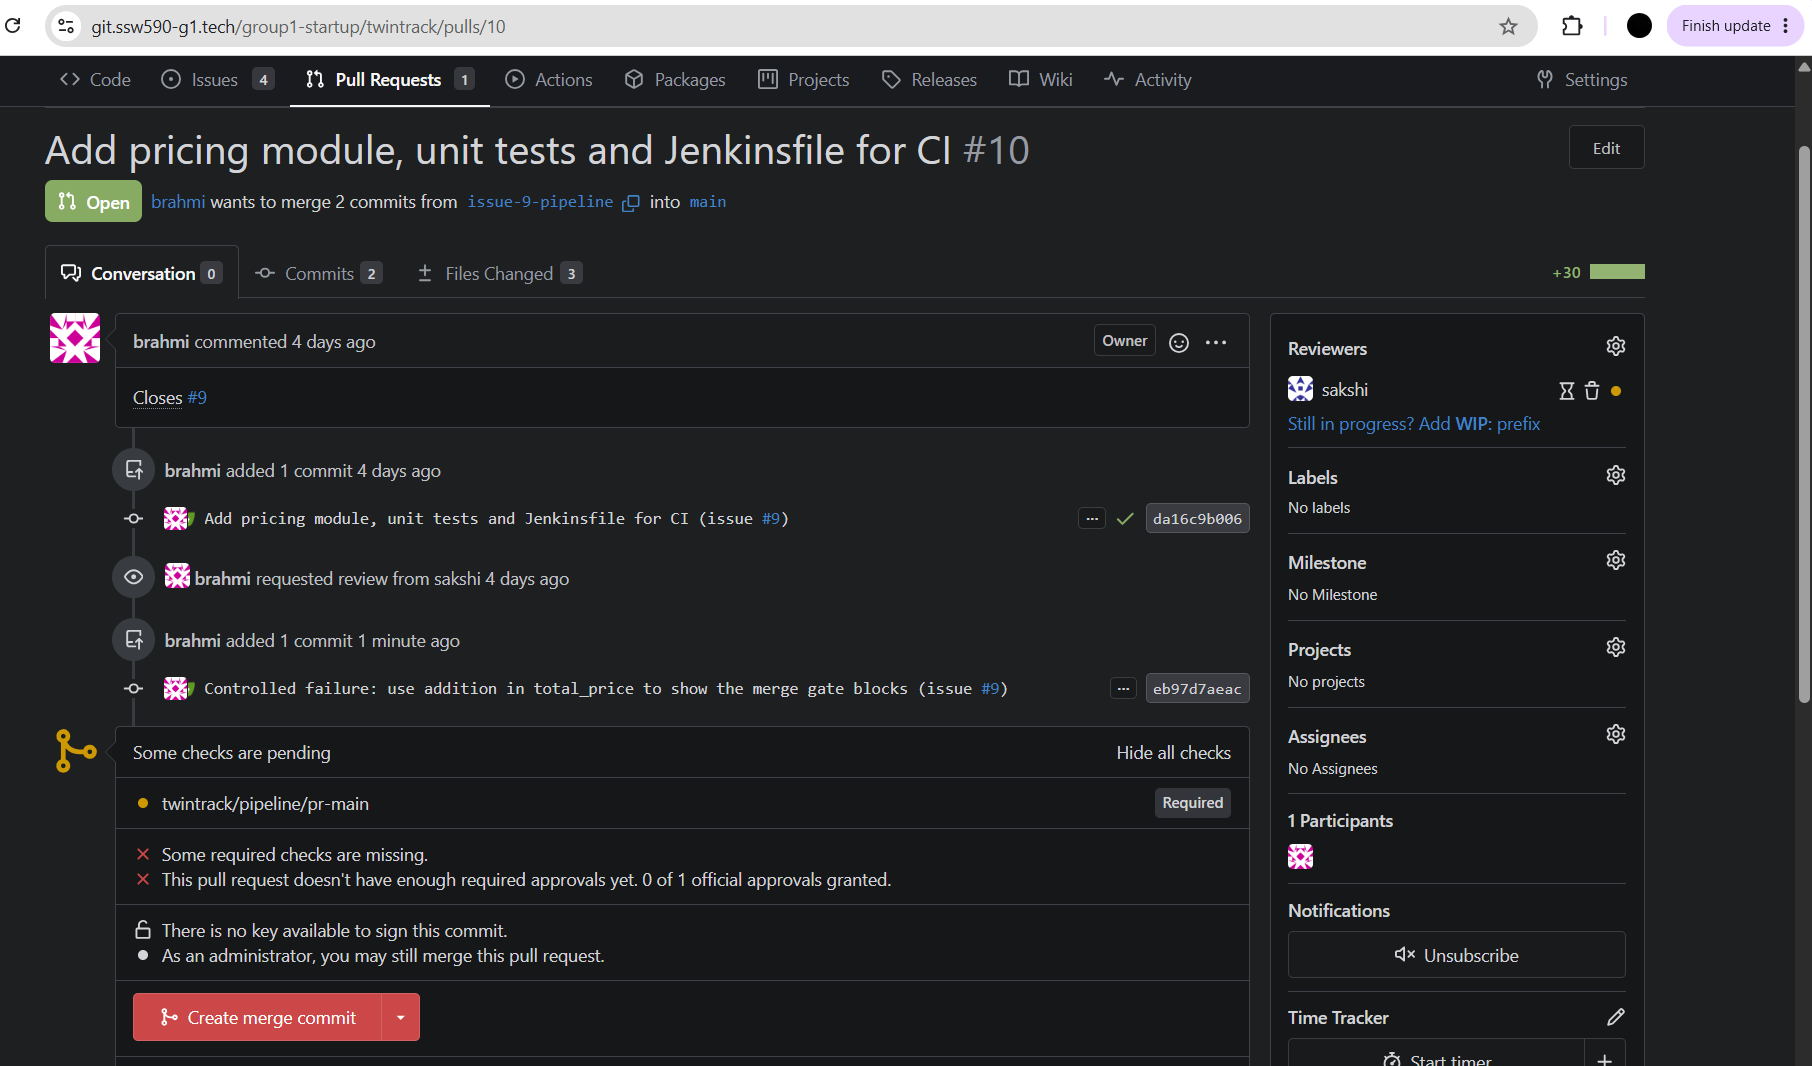
\includegraphics[width=\linewidth]{evidence/90-gitea-pr10-after-failing-push-required-check-pending-2026-11-02.png}
\caption{Pull request \#10 right after the first failing push (commit \texttt{eb97d7a}), November 2, 2026: the required check is marked \emph{Required} and still pending, with ``Some required checks are missing'' and ``0 of 1 official approvals''; the banner ``As an administrator, you may still merge'' is visible further down.}
\label{Fig:E90}
\end{figure}

% ======================================================================
% Region: jenkFailure (single owner; edit only your own region)
\subsection{Failure, repair, and review (10 points)}
\label{Section:jenkFailure}
\index{controlled failure}
\textbf{Owner:} SD. \textbf{Status:} two failures and repairs with matching IDs, peer review by SD, merge, and issue closure all observed;
checked by SD on November 3, 2026 against Gitea's pull-request timeline \StatusPass.

The work item is \href{\GiteaURL/group1-startup/twintrack/issues/9}{issue \#9} (``Add pricing module, unit tests and Jenkinsfile for CI'', \FigRef{71}) and the
pull request \href{\GiteaURL/group1-startup/twintrack/pulls/10}{\#10} with \texttt{Closes \#9} in its description, from branch \texttt{issue-9-pipeline}
into \texttt{main}. The controlled failure was made twice, the second time to capture the merge-gate screenshots with automatic builds.

\begin{figure}[htbp]
\centering
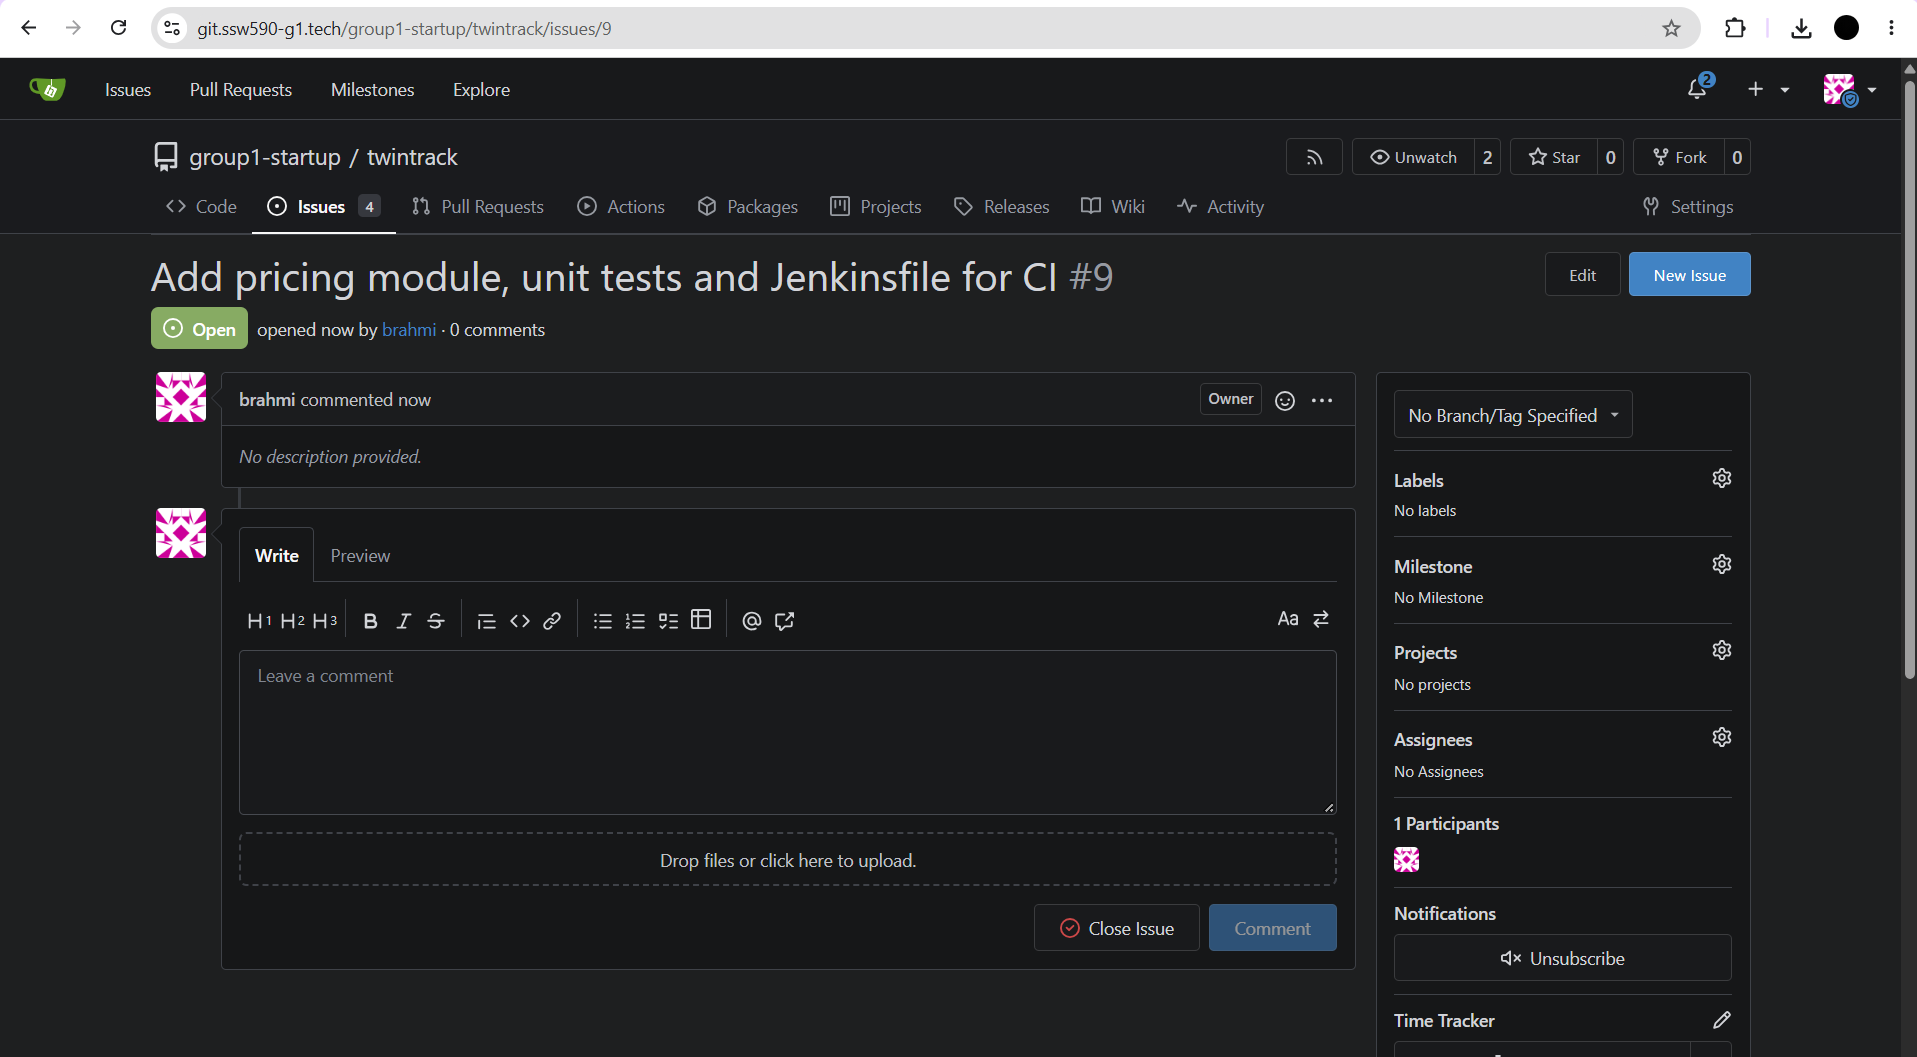
\includegraphics[width=0.85\linewidth]{evidence/71-gitea-twintrack-issue-9-pricing-jenkinsfile-opened-2026-10-29.png}
\caption{Issue \#9 in \texttt{twintrack}, opened October 29, 2026 by \texttt{brahmi}.}
\label{Fig:E71}
\end{figure}

\begin{tabularx}{\linewidth}{L{1.0cm}L{2.2cm}L{3.6cm}L{2.6cm}Y}
\caption{Dated sequence of commits and Jenkins builds for pull request \#10, October 29 to November 2, 2026\label{Table:JenkinsSequence}}\\
\toprule \textbf{Build} & \textbf{Commit} & \textbf{Change} & \textbf{Result} & \textbf{Started by, and evidence}\\ \midrule
\endfirsthead
\toprule \textbf{Build} & \textbf{Commit} & \textbf{Change} & \textbf{Result} & \textbf{Started by, and evidence}\\ \midrule
\endhead \bottomrule \endlastfoot
\#1 & \texttt{da16c9b} & bootstrap: Python example, tests, \texttt{Jenkinsfile} & success & repository scan (\ListRef{85})\\
\#2 & \texttt{eb97d7a} & controlled failure: addition instead of multiplication & \textbf{failure} (\texttt{13 != 30}) & started \emph{by hand} by BD (\ListRef{89}, \FigRef{90})\\
none & \texttt{7d7848f} & repair & \emph{never built} & the webhook lacked the Synchronized event (\ListRef{93})\\
\#3 & \texttt{d5e5c64} & no file change; proves the corrected webhook & success & \textbf{webhook} (\ListRef{94})\\
\#4 & \texttt{86ee9fc} & second controlled failure & \textbf{failure} (\texttt{13 != 30}) & \textbf{webhook} (\ListRef{96}, \FigRef{97})\\
\#5 & \texttt{92c121d} & repair: multiplication restored & success & \textbf{webhook} (\ListRef{99}, \FigRef{100})\\
review & \texttt{92c121d} & SD approves pull request \#10 with a review comment (00:51:00 UTC) & approved & SD in Gitea (\ListRef{106})\\
merge & \texttt{a0094a8} & SD merges \#10 into \texttt{main} (00:51:29 UTC); issue \#9 closes & merged & SD in Gitea (\ListRef{106})\\
\texttt{main} \#1 & \texttt{a0094a8} & Jenkins builds the merged \texttt{main} & success & \textbf{webhook} (\ListRef{106})\\
\end{tabularx}

\paragraph{Expected versus actual.} The test \texttt{test\_total} expects $10 \times 3 = 30$; with the broken line it computes 13, so the
\emph{Test} stage must fail and the required check must turn red. That is what builds \#2 and \#4 show (\ListRef{89}, \ListRef{96}); builds \#1, \#3 and \#5
pass. The final content of the pull request equals the original bootstrap (the diff between \texttt{da16c9b} and \texttt{92c121d} is empty).
The first demonstration was imperfect and is kept as a failed attempt, not hidden: build \#2 was started manually and the repair commit was never built, because of the
webhook event described in \ref{Section:jenkTrigger}; the second round was fully automatic. Nothing was done to the deployed Gitea or Jenkins services.

\paragraph{Push times and matching IDs.} Gitea's timeline of the pull request records every push with its commit
(\ListRef{107}): \texttt{da16c9b} on October 30, 00:07 UTC (October 29 US Eastern), then on November 3 (UTC) \texttt{eb97d7a} 00:14:34,
\texttt{7d7848f} 00:17:23, \texttt{d5e5c64} 00:24:27, \texttt{86ee9fc} 00:30:22, and \texttt{92c121d} 00:32:51. Each commit's statuses in Gitea
name the Jenkins run that produced them (\texttt{PR-10/2} for \texttt{eb97d7a}, \dots, \texttt{PR-10/5} for \texttt{92c121d}), which is how the IDs in
Table~\ref{Table:JenkinsSequence} are matched across the two systems. Two details a reader may notice: the second failure and its
repair were \emph{committed} one second apart (19:25:40 and 19:25:41 US Eastern) because both were prepared together, but they were
\emph{pushed} separately, two and a half minutes apart, so the failing commit was the pull request's head, and was tested and shown as
blocking, before the repair existed on the server. For \texttt{eb97d7a}, the first status appeared about two minutes after the push,
when BD started build \#2 by hand; for the webhook-started builds it appeared within three seconds of the push.

\begin{longlisting}
\inputminted[fontsize=\scriptsize]{text}{evidence/107-pr10-timeline-pushes-review-merge-and-commit-statuses-2026-11-03.txt}
\caption{Pull request \#10 from Gitea's API without a token, November 3, 2026: pushes with commit IDs, the review request,
SD's approval, the merge, issue \#9's closure, every commit status with its Jenkins run, and the branch rule (real output).}
\label{Listing:E107}
\end{longlisting}

\begin{longlisting}
\inputminted[fontsize=\scriptsize]{text}{evidence/96-jenkins-pr10-build-4-second-controlled-failure-webhook-triggered-2026-11-02.txt}
\caption{Build \#4, the second controlled failure (commit \texttt{86ee9fc}): cause, failing test, and Gitea statuses (real output).}
\label{Listing:E96}
\end{longlisting}

\begin{longlisting}
\inputminted[fontsize=\scriptsize]{text}{evidence/99-jenkins-pr10-build-5-repair-webhook-triggered-success-2026-11-02.txt}
\caption{Build \#5, the repair (commit \texttt{92c121d}): cause, passing tests, Gitea statuses, and all builds so far (real output).}
\label{Listing:E99}
\end{longlisting}

\begin{longlisting}
\inputminted[fontsize=\scriptsize]{text}{evidence/89-jenkins-pr10-build-2-controlled-failure-and-gitea-status-2026-11-02.txt}
\caption{Build \#2, the first controlled failure (commit \texttt{eb97d7a}), started manually, with the correction of an earlier wrong ``webhook-triggered'' label (real output).}
\label{Listing:E89}
\end{longlisting}

\paragraph{Peer review, merge, and closure.} Pull request \#10 was assigned for review to SD, the second member, on October 29, 2026, and Gitea required her
approval (\FigRef{100}, ``0 of 1 official approvals granted'' until then). On November 2, 2026 (19:51 US Eastern; 00:51 UTC on November 3) SD approved it
with a review comment: she checked the three files against the course manual, ran the tests and \texttt{py\_compile} locally (two tests \texttt{ok}), and
suggested a later test for a negative quantity. She merged it 29 seconds later as the merge commit \texttt{a0094a8}, and \textbf{issue \#9 closed automatically}
at the same moment (\ListRef{106}). The approval came from SD, the second member, not from the author BD, and it covered the head commit
\texttt{92c121d} that had passed the required check 18~minutes earlier; no commit was pushed between the passing check and the merge. The merge itself started a Jenkins build of \texttt{main} (build \#1 of the \texttt{main} job,
success in about 9 seconds, started by a branch event); its status context is \texttt{twintrack/pipeline/head}, because a build of a branch reports a
different context than a build of a pull request (\texttt{pr-main}), which is the one the branch rule requires.

\begin{longlisting}
\inputminted[fontsize=\scriptsize]{text}{evidence/106-pr10-review-merge-issue-closed-and-main-build-2026-11-02.txt}
\caption{Pull request \#10: SD's review and approval, the merge (commit \texttt{a0094a8}), issue \#9 closed automatically, and the Jenkins build of \texttt{main}, November 2, 2026 (real output).}
\label{Listing:E106}
\end{longlisting}

% ======================================================================
% Region: jenkBoundary (single owner; edit only your own region)
\subsection{Credentials and build boundary (10 points)}
\label{Section:jenkBoundary}
\textbf{Owner:} BD. \textbf{Status:} described from the observed configuration \StatusPass.

\begin{tabularx}{\linewidth}{L{3.3cm}L{3.4cm}Y}
\caption{Secrets and where they live (hints only, no values)\label{Table:JenkinsSecrets}}\\
\toprule \textbf{Secret} & \textbf{Stored in} & \textbf{Scope and handling}\\ \midrule
\endfirsthead
\toprule \textbf{Secret} & \textbf{Stored in} & \textbf{Scope and handling}\\ \midrule
\endhead \bottomrule \endlastfoot
Jenkins one-time unlock password & the Jenkins volume on the server only & Read once on the server to finish setup; never copied anywhere\\
Jenkins account passwords (\texttt{brahmi}, \texttt{sakshi}) & password managers of the owners & Sakshi received a temporary password privately and changes it at first sign-in; sign-up is closed\\
\texttt{jenkins-bot} Gitea token & Jenkins credential store (\texttt{gitea-jenkins-bot}) & Narrow scopes; Write only on \texttt{twintrack}; to be deleted after grading\\
Webhook secret & none & The webhook only travels over the private Docker network and Jenkins is not reachable from outside; this is a stated limitation\\
Team address list & the server's untracked \texttt{.env}, mode 600 & Not in the repository, the compose file, or this PDF\\
\end{tabularx}

\paragraph{Who can change the Jenkinsfile.} Anyone with write access to \texttt{twintrack}: BD and SD (and the integration user, which only reads and reports).
Because \texttt{main} is protected, a change to the \texttt{Jenkinsfile} reaches \texttt{main} only through a pull request with one approval and a passing required check.
Registration on Gitea is closed, so there are no outside accounts that could open a pull request.

\paragraph{Where builds run and the specific risk.} Builds run on the \textbf{Jenkins controller executor}, inside the Jenkins container, not on a separate agent
(allowed by the course manual for a small deployment \cite{JenkinsControllerIsolation,DosManual}). The risk: pipeline code is run on the same process that holds
Jenkins' credentials and configuration, so a malicious pipeline could read them \cite{JenkinsCredentials,JenkinsSecurity}. Compensating restrictions: only two trusted
people can change pipeline code; no outsiders can create accounts or pull requests; the example pipeline uses no credentials step and no repository secret; the
container has no Docker socket and is not privileged; its memory is limited; and Jenkins is not reachable from the internet beyond the login page. Untrusted pull
requests therefore cannot obtain secrets or privileged Docker access because there are no untrusted contributors in this deployment.

\paragraph{Plugin-update check and operator response.} On November 2, 2026 the 60 installed plugins and the core were compared with Jenkins' stable update
center: the core (2.580.2) is current; one plugin has a newer version (\texttt{workflow-cps}); and no advisory applies to any installed version (\ListRef{104}). No update
was applied days before the deadline, to avoid breaking a working, evidenced pipeline; it would be applied after submission by rebuilding the image. A first count of ``78 warnings'' was wrong
(historical advisories) and is corrected in the same listing.

\begin{longlisting}
\inputminted[fontsize=\scriptsize]{text}{evidence/104-jenkins-plugin-and-core-update-check-2026-11-02.txt}
\caption{Plugin and core update check against the stable update center, November 2, 2026 (real output).}
\label{Listing:E104}
\end{longlisting}

\paragraph{Troubleshooting a failed webhook or build.}
\begin{enumerate}
\item \emph{No build started after a push:} check the webhook's Recent Deliveries in Gitea, then Jenkins' Multibranch Pipeline Events; confirm the events ticked include Pull Request Synchronized; use Scan Repository Now as a fallback.
\item \emph{Build red:} open the build's console; the failing stage and the assertion are printed; reproduce with \texttt{python -m unittest discover -s tests -v}.
\item \emph{Status not on the pull request:} check that the Jenkins credential still works and that \texttt{jenkins-bot} still has Write; the status context must read \texttt{twintrack/pipeline/pr-main}.
\item \emph{Jenkins slow or killed:} look at memory and swap on the server (\texttt{free -m}); Jenkins is limited to 640~MiB; restart only the Jenkins container with \texttt{docker compose restart jenkins}.
\item \emph{Locked out of the dashboard:} the team address in \texttt{.env} may have changed; update it and recreate Caddy.
\end{enumerate}

% ======================================================================
% Region: jenkQuality (single owner; edit only your own region)
\subsection{Manual quality and controls (10 points)}
\label{Section:jenkQuality}
\index{Jenkins!quality controls}
\textbf{Owner:} SD. \textbf{Status:} drafted by BD and Claude Code; checked and completed by SD on November 3, 2026
(activity diagram, citation check, troubleshooting pointer, evidence 107--108) \StatusPass.

\paragraph{Version, history, and tables.} The manual's version is increased from 1.1 to \textbf{1.2}. A dated history entry for this update links this chapter and names
the Hosts and Passwords changes (\ref{Table:DocumentHistory}). \textbf{Hosts and Passwords tables: changed} (\ChapterRef{HostsPasswords}): a Jenkins row in Hosts,
the \texttt{ci} DNS record, and Passwords hints for the Jenkins accounts, the \texttt{jenkins-bot} user and token, the webhook (no secret), and the team address list;
no secret is recorded. Figure~\ref{Figure:JenkinsDeployment} is the adapted UML deployment diagram. New glossary and index terms: Jenkins, Jenkinsfile, webhook,
status check, controller executor, multibranch pipeline. Citations are listed in the bibliography. On November 3, 2026, SD opened each cited Jenkins and Gitea page
(Jenkins Docker installation, Gitea plugin, Gitea Checks plugin, security, credentials, controller isolation; Gitea webhooks and
protected branches): all were available, and the protected-branches page was checked for the two claims this chapter makes with it,
required status checks and approvals, and the administrator-override option \cite{GiteaProtectedBranches}.

\paragraph{Operator restart note.} Restart Jenkins with \texttt{docker compose restart jenkins} in \texttt{\textasciitilde/jenkins} (ready in about 13 seconds,
data kept); restart Caddy only with \texttt{docker compose up -d caddy} in \texttt{\textasciitilde/gitea} after validating the Caddyfile; Gitea needs about 40 seconds to be healthy.
Both services restart on their own after a reboot (\texttt{unless-stopped}).

\paragraph{Operator troubleshooting note.} If a pull request shows no status or the wrong one, follow the procedure in
Section~\ref{Section:jenkBoundary}. The three checks that found this assignment's real problems are, in order: (1) the pull request's
commit list in Gitea, where every head commit should get a \texttt{twintrack/pipeline/pr-main} status within seconds of its push
(\ListRef{107}); a commit with none was never built, as with \texttt{7d7848f}; (2) the repository webhook's recent deliveries and its event
selection, which must include \emph{Pull Request Synchronized} (\FigRef{92}); (3) the failing Jenkins run's console, where the first
assertion or error names the cause (\texttt{13 != 30} in builds \#2 and \#4).

\paragraph{Activity diagram.} Figure~\ref{Figure:JenkinsActivity} is the course's pull-request-to-merge activity
(manual Figure~4.1) annotated with what actually happened on pull request \#10. The webhook starts a run, but the merge is gated by
the required check reported on the latest head commit, and a passing check still needed SD's approval before the merge.

\begin{figure}[htbp]
\centering
\resizebox{0.95\linewidth}{!}{% Owner: SD. Activity diagram of the pull-request-to-merge flow, adapted from the course manual's Figure 4.1
% and annotated with the real commits, Jenkins builds and times of pull request #10 (UTC, Nov 3 unless noted).
% Included by devopsJenkins.tex (jenkQuality region). Only the tikzpicture lives here.
\begin{tikzpicture}[
  font=\footnotesize, >={Stealth[length=2.2mm]},
  base/.style={draw, rounded corners=3pt, align=center, text width=5.0cm, inner sep=4pt},
  act/.style={base, fill=devopsLightBlue},
  dec/.style={base, rounded corners=10pt, fill=yellow!12},
  bad/.style={base, fill=red!8},
  good/.style={base, fill=green!8}]
  \node[act] (open) at (0,0) {Open issue-linked PR \#10 (\texttt{Closes \#9}) to protected \texttt{main}\\[1pt]
    {\scriptsize\itshape commit \texttt{da16c9b} (Oct 29); build \#1 success (Nov 2)}};
  \node[act] (hook) at (0,-2.0) {Gitea sends the webhook\\(Pull Request Synchronized)\\[1pt]
    {\scriptsize\itshape builds \#3--\#5 by webhook; \#2 by hand;\\ \texttt{7d7848f} never built (event missing)}};
  \node[act] (build) at (0,-4.2) {Jenkins checks out the PR head merged with \texttt{main};\\\texttt{py\_compile}, \texttt{unittest}};
  \node[act] (report) at (0,-6.0) {\texttt{jenkins-bot} reports\\\texttt{twintrack/pipeline/pr-main}\\[1pt]
    {\scriptsize\itshape pending 2--3\,s after each push}};
  \node[dec] (pass) at (0,-8.0) {Required check passes\\on the latest PR head?};
  \node[good] (review) at (0,-10.0) {Yes: team reviews the PR\\[1pt]
    {\scriptsize\itshape after \texttt{92c121d} (\#5) success 00:33:18}};
  \node[dec] (appr) at (0,-12.0) {Review approved?\\[1pt]{\scriptsize\itshape SD approved 00:51:00, with a comment}};
  \node[good] (merge) at (0,-14.1) {Yes: merge PR into \texttt{main}\\[1pt]
    {\scriptsize\itshape \texttt{a0094a8} 00:51:29; issue \#9 closed;\\ \texttt{main} build \#1 (\texttt{pipeline/head}) success}};

  \node[bad] (blocked) at (7.0,-8.0) {No: merge blocked\\[1pt]
    {\scriptsize\itshape \texttt{eb97d7a} (\#2), \texttt{86ee9fc} (\#4):\\ \texttt{13 != 30}, ``Some required checks failed''}};
  \node[bad] (fix) at (7.0,-10.0) {Fix the failure; push a new commit\\[1pt]
    {\scriptsize\itshape repairs \texttt{7d7848f}, then \texttt{92c121d}}};
  \node[bad] (revise) at (7.0,-12.0) {No: revise; push a new commit\\[1pt]{\scriptsize\itshape not needed for PR \#10}};

  \foreach \a/\b in {open/hook, hook/build, build/report, report/pass, pass/review, review/appr, appr/merge} \draw[->, thick] (\a) -- (\b);
  \draw[->, thick] (pass) -- node[above, font=\scriptsize] {no} (blocked);
  \draw[->, thick] (blocked) -- (fix);
  \draw[->, thick] (appr) -- node[above, font=\scriptsize] {no} (revise);
  \draw[->, thick] (fix.east) -- ++(0.6,0) |- (hook.east);
  \draw[thick] (revise.east) -- ++(0.6,0) -- ++(0,2.0);
\end{tikzpicture}
}
\caption{Pull-request-to-merge activity for pull request \#10, adapted from the course manual's Figure~4.1 \cite{DosManual} with the real
commits, Jenkins builds, and times (UTC, November 3, 2026, unless noted; \ListRef{107}). A new commit repeats the build; the check on the
latest head commit, not the webhook delivery, gates the merge.}
\label{Figure:JenkinsActivity}
\end{figure}

\begin{tabularx}{\linewidth}{L{0.8cm}L{5.1cm}Y}
\caption{Failed tests and mistakes of this assignment, and the corrections\label{Table:JenkinsFailed}}\\
\toprule \textbf{\#} & \textbf{What went wrong} & \textbf{Correction and evidence}\\ \midrule
\endfirsthead
\toprule \textbf{\#} & \textbf{What went wrong} & \textbf{Correction and evidence}\\ \midrule
\endhead \bottomrule \endlastfoot
1 & The webhook was first created in BD's personal account settings, so it never fired for the organization's repository & Recreated on the repository (\FigRef{86})\\
2 & The webhook lacked the Pull Request Synchronized event: pushes reached Jenkins but no build was scheduled; the repair commit \texttt{7d7848f} was never built & Diagnosed from \ListRef{93} and \FigRef{92}; fixed; proven by build \#3 (\ListRef{94})\\
3 & Build \#2 was started by hand while the webhook did not work; an earlier evidence file wrongly called it webhook-triggered & Corrected in \ListRef{89}\\
4 & The first reading of the restart time (9 seconds) matched the previous start's log line, and \texttt{/login} answered 503 at that moment & Re-measured: about 12.6 seconds (\ListRef{102})\\
5 & A first plugin check counted 78 historical advisories as findings & Re-tested against the installed versions: 0 apply (\ListRef{104})\\
6 & A 403 at \texttt{/} seen from the team address was first taken for Caddy's block & Headers showed Jenkins' own response (\ListRef{75})\\
7 & The first push of a test commit to Gitea failed (``Authentication failed'') because a deleted token was still saved in the Git credential store & Saved sign-in cleared and replaced; no secret was exposed\\
8 & The repository owner could override the merge rule (``As an administrator, you may still merge'') & Accepted and disclosed (\FigRef{90}); not enabled to block administrators\\
\end{tabularx}

\paragraph{Limitations stated plainly.} The first real renewal of the Jenkins certificate has not happened. The restart test shows persistence, not backup. The security
group probes of 8080, 50000, and 3000 ran from the administrator's computer. The merge button area is outside the cropped screenshot of the blocked state. The
webhook has no secret. The peer review of pull request \#10 was a single review by SD (one required approval), and her suggestion for a negative-quantity test was
not implemented. Jenkins shares a 1~GB host with Gitea and has little memory headroom.
